
\chapter{Process safety and instrumentation}

This chapter discusses instrumentation issues related to industrial process safety.  Instrumentation safety may be broadly divided into two categories: how instruments themselves may pose a safety hazard (electrical signals possibly igniting hazardous atmospheres), and how instruments and control systems may be configured to detect unsafe process conditions and automatically shut an unsafe process down.

In either case, the intent of this chapter is to help define and teach how to mitigate hazards encountered in certain instrumented processes.  I purposely use the word ``mitigate'' rather than ``eliminate'' because the complete elimination of all risk is an impossibility.  Despite our best efforts and intentions, no one can absolutely eliminate all dangers from industrial processes\footnote{For that matter, it is impossible to eliminate all danger from \textit{life in general}.  Every thing you do (or don't do) involves some level of risk.  The question really should be, ``how much risk is there in a given action, and how much risk am I willing to tolerate?''  To illustrate, there does exist a non-zero probability that something you will read in this book is so shocking it will cause you to suffer a heart attack.  However, the odds of you walking away from this book and never reading it again over concern of epiphany-induced cardiac arrest are just as slim.}.  What we can do, though, is \textit{significantly} reduce those risks to the point they begin to approach the low level of ``background'' risks we all face in daily life, and that is no small achievement.

\vskip 10pt

An important philosophy to follow in the safe design is something called \textit{defense-in-depth}.  This is the principle of using multiple layers\footnote{Also humorously referred to as the ``belt \textit{and} suspenders'' school of engineering.} of protection, in case one or more of those layers fail.  Applying defense-in-depth to process design means regarding each and every safety tool and technique as part of a multi-faceted strategy, rather than as a set of mutually-exclusive alternatives.  \index{Defense-in-depth}

To give a brief example of defense-in-depth applied to overpressure protection in a fluid processing system, that system might defend against excessive fluid pressure using all of the following techniques:

\begin{itemize}
\item A pressure-control system with an operator-adjusted setpoint
\item High-pressure alarms to force operator attention 
\item A safety shutdown system triggered by abnormally high pressure
\item Temperature control systems (both regulatory and safety shutdown) to prevent excessive temperature from helping to create excessive fluid pressure
\item Pressure-relief valves which automatically open to vent high pressure
\item Pressure vessels built with ``frangible\footnote{Frangible roofs are a common design applied to liquid storage tanks harboring the potential for overpressure, such as sulfuric acid storage tanks which may generate accumulations of explosive hydrogen gas.  Having the roof seam rupture from overpressure is a far less destructive event than having a side seam or floor seam rupture and consequently spill large volumes of acid.  This technique of mitigating overpressure risk does not work to reduce pressure in the system, but it does reduce the risk of damage caused by overpressure in the system.}'' tops designed to burst in the safest manner possible
\item Locating the process far away from anything (or anyone) that might be harmed by an overpressure event
\end{itemize}

Any one of these techniques will work to reduce the risk posed by excessive fluid pressure in the system, but all of them used together will provide greater risk reduction than any one used alone.






\filbreak
\section{Classified areas and electrical safety measures}

Any physical location in an industrial facility harboring the potential of explosion due to the presence of flammable process matter suspended in the air is called a \textit{hazardous} or \textit{classified} location.  In this context, the label ``hazardous'' specifically refers to the hazard of explosion, not of other health or safety hazards\footnote{Chemical corrosiveness, biohazardous substances, poisonous materials, and radiation are all examples of other types of industrial hazards not covered by the label ``hazardous'' in this context.  This is not to understate the danger of these other hazards, but merely to focus our attention on the specific hazard of explosions and how to build instrument systems that will not trigger explosions due to electrical spark.}.  \index{Hazardous location}  \index{Classified location}






\filbreak
\subsection{Classified area taxonomy}

\label{classified_areas}

In the United States, the National Electrical Code (NEC) published by the National Fire Protection Association (NFPA) defines different categories of ``classified'' industrial areas and prescribes safe electrical system design practices for those areas.  Article 500 of the NEC categorizes classified areas into a system of \textit{Classes} and \textit{Divisions}.  Articles 505 and 506\footnote{Article 506 is a new addition to the NEC as of 2008.  Prior to that, the only ``zone''-based categories were those specified in Article 505.} of the NEC provide alternative categorizations for classified areas based on \textit{Zones} that is more closely aligned with European safety standards.  \index{National Electrical Code (NEC)}  \index{National Fire Protection Association (NFPA)}  \index{NEC}

The Class and Division taxonomy defines classified areas in terms of hazard type and hazard probability.  Each ``Class'' contains (or may contain) different types of potentially explosive substances: Class I is for gases or vapors, Class II is for combustible dusts, and Class III is for flammable fibers.  The three-fold class designation is roughly scaled on the size of the flammable particles, with Class I being the smallest (gas or vapor molecules) and Class III being the largest (fibers of solid matter).  Each ``Division'' ranks a classified area according to the likelihood of explosive gases, dusts, or fibers being present.  Division 1 areas are those where explosive concentrations can or do exist under normal operating conditions.  Division 2 areas are those where explosive concentrations only exist infrequently or under abnormal conditions\footnote{The final authority on Class and Division definitions is the National Electrical Code itself.  The definitions presented here, especially with regard to Divisions, may not be precise enough for many applications.  Article 500 of the NEC is quite specific for each Class and Division combination, and should be referred to for detailed information in any particular application.}.  \index{Class, hazardous area}  \index{Division, hazardous area}

The ``Zone'' method of area classifications defined in Article 505 of the National Electrical Code applies to Class I (explosive gas or vapor) applications, but the three-fold Zone ranks (0, 1, and 2) are analogous to Divisions in their rating of explosive concentration probabilities.  Zone 0 defines areas where explosive concentrations are continually present or normally present for long periods of time.  Zone 1 defines areas where those concentrations may be present under normal operating conditions, but not as frequently as Zone 0.  Zone 2 defines areas where explosive concentrations are unlikely under normal operating conditions, and when present do not exist for substantial periods of time.  This three-fold Zone taxonomy may be thought of as expansion on the two-fold Division system, where Zones 0 and 1 are sub-categories of Division 1 areas, and Zone 2 is nearly equivalent to a Division 2 area\footnote{Once again, the final authority on this is the National Electrical Code, in this case Article 505.  My descriptions of Zones and Divisions are for general information only, and may not be specific or detailed enough for many applications.}.  A similar three-zone taxonomy for Class II and Class III applications is defined in Article 506 of the National Electrical Code, the zone ranks for these dust and fiber hazards numbered 20, 21, and 22 (and having analogous meanings to zones 0, 1, and 2 for Class I applications).  \index{Zone, hazardous area}

An example of a classified area common to most peoples' experience is a vehicle refueling station.  Being a (potentially) explosive \textit{vapor}, the hazard in question here is deemed Class I.  The Division rating varies with proximity to the fume source.  For an upward-discharging vent pipe from an underground gasoline storage tank, the area is rated as Division 1 within 900 millimeters (3 feet) from the vent hole.  Between 3 feet and 5 feet away from the vent, the area is rated as Division 2.  In relation to an outdoor fuel pump (dispenser), the space internal to the pump enclosure is rated Division 1, and any space up to 18 inches from grade level and up to 20 feet away (horizontally) from the pump is rated Division 2.

\filbreak

Within Class I and Class II (but not Class III), the National Electrical Code further sub-divides hazards according to explosive properties called \textit{Groups}.  Each group is defined either according to a substance type, or according to specific ignition criteria.  Ignition criteria listed in the National Electrical Code (Article 500) include the \textit{maximum experimental safe gap} (MESG) and the \textit{minimum ignition current ratio} (MICR).  The MESG is based on a test where two hollow hemispheres separated by a small gap enclose both an explosive air/fuel mixture and an ignition source.  Tests are performed with this apparatus to determine the maximum gap width between the hemispheres that will not permit the excursion of flame from an explosion within the hemispheres triggered by the ignition source.  The MICR is the ratio of electrical ignition current for an explosive air/fuel mixture compared to an optimum mixture of methane and air.  The smaller of either these two values, the more dangerous the explosive substance is.  \index{Maximum experimental safe gap (MESG)}  \index{Minimum ignition current ratio (MICR)}  \index{Group, hazardous area}

\vskip 10pt

Class I substances are grouped according to their respective MESG and MICR values, with typical gas types given for each group: 

% No blank lines allowed between lines of an \halign structure!
% I use comments (%) instead, so that TeX doesn't choke.

$$\vbox{\offinterlineskip
\halign{\strut
\vrule \quad\hfil # \ \hfil & 
\vrule \quad\hfil # \ \hfil & 
\vrule \quad\hfil # \ \hfil & 
\vrule \quad\hfil # \ \hfil \vrule \cr
\noalign{\hrule}
%
% First row
\textbf{Group} & \textbf{Typical substance} & \textbf{Safe gap} & \textbf{Ignition current} \cr
%
\noalign{\hrule}
%
% Another row
A & Acetylene &  &  \cr
%
\noalign{\hrule}
%
% Another row
B & Hydrogen & MESG $\leq$ 0.45 mm & MICR $\leq$ 0.40 \cr
%
\noalign{\hrule}
%
% Another row
C & Ethylene & 0.45 mm $<$ MESG $\leq$ 0.75 mm & 0.40 $<$ MICR $\leq$ 0.80 \cr
%
\noalign{\hrule}
%
% Another row
D & Propane & 0.75 mm $<$ MESG & 0.80 $<$ MICR \cr
%
\noalign{\hrule}
} % End of \halign 
}$$ % End of \vbox

\vskip 10pt

Class II substances are grouped according to material type:

% No blank lines allowed between lines of an \halign structure!
% I use comments (%) instead, so that TeX doesn't choke.

$$\vbox{\offinterlineskip
\halign{\strut
\vrule \quad\hfil # \ \hfil & 
\vrule \quad\hfil # \ \hfil \vrule \cr
\noalign{\hrule}
%
% First row
\textbf{Group} & \textbf{Substances} \cr
%
\noalign{\hrule}
%
% Another row
E & Metal dusts \cr
%
\noalign{\hrule}
%
% Another row
F & Carbon-based dusts \cr
%
\noalign{\hrule}
%
% Another row
G & Other dusts (wood, grain, flour, plastic, etc.) \cr
%
\noalign{\hrule}
} % End of \halign 
}$$ % End of \vbox

\vskip 10pt

Just to make things confusing, the Class/Zone system described in NEC Article 505 uses a completely different lettering order to describe gas and vapor groups (at the time of this writing there is no grouping of dust or fiber types for the zone system described in Article 506 of the NEC):

% No blank lines allowed between lines of an \halign structure!
% I use comments (%) instead, so that TeX doesn't choke.

$$\vbox{\offinterlineskip
\halign{\strut
\vrule \quad\hfil # \ \hfil & 
\vrule \quad\hfil # \ \hfil & 
\vrule \quad\hfil # \ \hfil & 
\vrule \quad\hfil # \ \hfil \vrule \cr
\noalign{\hrule}
%
% First row
\textbf{Group} & \textbf{Typical substance(s)} & \textbf{Safe gap} & \textbf{Ignition current} \cr
%
\noalign{\hrule}
%
% Another row
IIC & Acetylene, Hydrogen & MESG $\leq$ 0.50 mm & MICR $\leq$ 0.45 \cr
%
\noalign{\hrule}
%
% Another row
IIB & Ethylene & 0.50 mm $<$ MESG $\leq$ 0.90 mm & 0.45 $<$ MICR $\leq$ 0.80 \cr
%
\noalign{\hrule}
%
% Another row
IIA & Acetone, Propane & 0.90 mm $<$ MESG & 0.80 $<$ MICR \cr
%
\noalign{\hrule}
} % End of \halign 
}$$ % End of \vbox







\filbreak
\subsection{Explosive limits}

In order to have combustion (an explosion being a particularly aggressive form of combustion), certain basic criteria must be satisfied: a proper \textit{oxidizer/fuel ratio}, sufficient \textit{energy} for ignition, and the \textit{potential for a self-sustaining chemical reaction} (i.e. the absence of any chemical inhibitors).  We may show these criteria in the form of a \textit{fire triangle}\footnote{Traditionally, the three elements of a ``fire triangle'' were fuel, oxidizer, and ignition source.  However, this model fails to account for fuels not requiring oxygen as well as cases where a chemical inhibitor prevents a self-sustaining reaction even in the presence of fuel, oxidizer, and ignition source.}, the concept being that removing any of these three critical elements renders a fire (or explosion) impossible:  \index{Fire triangle}

$$
\includegraphics{safe_05.eps}$$

The fire triangle serves as a qualitative guide for \textit{preventing} fires and explosions, but it does not give sufficient information to tell us if the necessary conditions exist to \textit{support} a fire or explosion.  In order for a fire or explosion to occur, we need to have an adequate mixture of fuel and oxidizer in the correct proportions, and a source of ignition energy exceeding a certain minimum threshold.

\vskip 10pt

Suppose we had a laboratory test chamber filled with a mixture of acetone vapor (70\% by volume) and air at room temperature, with an electrical spark gap providing convenient ignition.  No matter how energetic the spark, this mixture would not explode, because there is too \textit{rich} a mixture of acetone (i.e. too much acetone mixed with not enough air).  Every time the spark gap discharges, its energy would surely cause some acetone molecules to combust with available oxygen molecules.  However, since the air is so dilute in this rich acetone mixture, those scarce oxygen molecules are depleted fast enough that the flame temperature quickly falls off and is no longer hot enough to trigger the remaining oxygen molecules to combust with the plentiful acetone molecules.  \index{Over-rich condition}

The same problem occurs if the acetone/air mixture is too \textit{lean} (not enough acetone and too much air).  This is what would happen if we diluted the acetone vapors to a volumetric concentration of only 0.5\% inside the test chamber: any spark at the gap would indeed cause some acetone molecules to combust, but there would be too few available to support expansive combustion across the rest of the chamber.  \index{Over-lean condition}

We could also have an acetone/air mixture in the chamber ideal for combustion (about 9.5\% acetone by volume) and still not have an explosion if the spark's energy were insufficient.  Most combustion reactions require a certain minimum level of \textit{activation energy} to overcome the potential barrier before molecular bonding between fuel atoms and oxidizer atoms occurs.  Stated differently, many combustion reactions are not \textit{spontaneous} at room temperature and at atmospheric pressure -- they need a bit of ``help'' to initiate.

\filbreak

All the necessary conditions for an explosion (assuming no chemical inhibitors are present) may be quantified and plotted as an \textit{ignition curve} for any particular fuel and oxidizer combination.  This next graph shows an ignition curve for an hypothetical fuel gas mixed with air:

$$\includegraphics{safe_06.eps}$$

Note how any point in the chart lying \textit{above} the curve is ``dangerous,'' while any point \textit{below} the curve is ``safe.''  The three critical values on this graph are the \textit{Lower Explosive Limit} (LEL), the \textit{Upper Explosive Limit} (UEL), and the \textit{Minimum Ignition Energy} (MIE).  These critical values differ for every type of fuel and oxidizer combination, change with ambient temperature and pressure, and may be rendered irrelevant in the presence of a catalyst (a chemical substance that works to promote a reaction without itself being consumed by the reaction).  Most ignition curves are published with the assumed conditions of air as the oxidizer, at room temperature and atmospheric pressure, with no catalyst(s) present.  \index{Lower explosive limit (LEL)}  \index{LEL}  \index{Upper explosive limit}  \index{UEL}  \index{Minimum Ignition Energy}  \index{MIE}

Some substances are so reactive that their minimum ignition energy (MIE) levels are well below the thermal energy of ambient air temperatures.  Such fuels will \textit{auto-ignite} the moment they come into contact with air, which effectively means one cannot prevent a fire or explosion by eliminating sources of flame or sparks.  When dealing with such substances, the only means for preventing fires and explosions lies with maintaining fuel/air ratios outside of the danger zone (i.e. below the LEL or above the UEL), or by using a chemical inhibitor to prevent a self-sustaining reaction.

\filbreak

The greater the difference in LEL and UEL values, the greater ``explosive potential'' a fuel gas or vapor presents (all other factors being equal), because it means the fuel may explode over a wider range of mixture conditions.  It is instructive to research the LEL and UEL values for many common substances, just to see how ``explosive'' they are relative to each other:

% No blank lines allowed between lines of an \halign structure!
% I use comments (%) instead, so that TeX doesn't choke.

$$\vbox{\offinterlineskip
\halign{\strut
\vrule \quad\hfil # \ \hfil & 
\vrule \quad\hfil # \ \hfil & 
\vrule \quad\hfil # \ \hfil \vrule \cr
\noalign{\hrule}
%
% First row
\textbf{Substance} & \textbf{LEL} (\% volume) & \textbf{UEL} (\% volume) \cr
%
\noalign{\hrule}
%
% Another row
Acetylene & 2.5\% & 100\% \cr
%
\noalign{\hrule}
%
% Another row
Acetone & 2.5\% & 12.8\% \cr
%
\noalign{\hrule}
%
% Another row
Butane & 1.5\% & 8.5\% \cr
%
\noalign{\hrule}
%
% Another row
Carbon disulfide & 1.3\% & 50\% \cr
%
\noalign{\hrule}
%
% Another row
Carbon monoxide & 12.5\% & 74\% \cr
%
\noalign{\hrule}
%
% Another row
Ether & 1.9\% & 36\% \cr
%
\noalign{\hrule}
%
% Another row
Ethylene oxide & 2.6\% & 100\% \cr
%
\noalign{\hrule}
%
% Another row
Gasoline & 1.4\% & 7.6\% \cr
%
\noalign{\hrule}
%
% Another row
Kerosene & 0.7\% & 5\% \cr
%
\noalign{\hrule}
%
% Another row
Hydrazine & 2.9\% & 98\% \cr
%
\noalign{\hrule}
%
% Another row
Hydrogen & 4.0\% & 74.2\% \cr
%
\noalign{\hrule}
%
% Another row
Methane & 4.4\% & 17\% \cr
%
\noalign{\hrule}
%
% Another row
Propane & 2.1\% & 9.5\% \cr
%
\noalign{\hrule}
} % End of \halign 
}$$ % End of \vbox

Note how both acetylene and ethylene oxide have UEL values of 100\%.  This means it is possible for these gases to explode \textit{even when there is no oxidizer present}.  Some other chemical substances exhibit this same property (n-propyl nitrate being another example), where the lack of an oxidizer does not prevent an explosion.  With these substances in high concentration, our only practical hope of avoiding explosion is to eliminate the possibility of an ignition source in its presence.  Some substances have UEL values so high that the elimination of oxidizers is only an uncertain guard against combustion: hydrazine being one example with a UEL of 98\%, and diborane being another example with a UEL of 88\%.  








%\filbreak
%\subsection{Electrical parameters}

% ADD: energy stored in a capacitor
% ADD: energy stored in an inductor
% ADD: ignition curves for different explosive air mixtures









\filbreak
\subsection{Protective measures}

Different strategies exist to help prevent electrical devices from triggering fires or explosions in classified areas.  These strategies may be broadly divided four ways: 

\begin{itemize}
\item \textbf{Contain the explosion:} enclose the device inside a very strong box that contains any explosion generated by the device so as to not trigger a larger explosion outside the box.  This strategy may be viewed as eliminating the ``ignition'' component of the fire triangle, from the perspective of the atmosphere outside the explosion-proof enclosure (ensuring the explosion inside the enclosure does not ignite a larger explosion outside).
\item \textbf{Shield the device:} enclose the electrical device inside a suitable box or shelter, then purge that enclosure with clean air (or a pure gas) that prevents an explosive mixture from forming inside the enclosure.  This strategy works by eliminating the ``proper fuel/oxidizer ratio'' component of the fire triangle: by eliminating fuel (if purged by air), or by eliminating oxidizer (if purged by fuel gas), or by eliminating both (if purged by an inert gas).
\item \textbf{Encapsulated design:} manufacture the device so that it is self-enclosing.  In other words, build the device in such a way that any spark-producing elements are sealed air-tight within the device from any explosive atmosphere.  This strategy works by eliminating the ``ignition'' component of the fire triangle (from the perspective of outside the device) or by eliminating the ``proper fuel/oxidizer ratio'' component (from the perspective of inside the device).
\item \textbf{Limit total circuit energy:} design the circuit such that there is insufficient energy to trigger an explosion, even in the event of an electrical fault.  This strategy works by eliminating the ``ignition'' component of the fire triangle.
\end{itemize}

It should be noted that any one of these strategies, correctly and thoroughly applied, is sufficient to mitigate the risk of fire and explosion.  For this reason you will seldom see more than one of these strategies simultaneously applied (e.g. an explosion-proof enclosure housing a circuit with insufficient energy to trigger an explosion).

\filbreak

A common example of the first strategy is to use extremely rugged metal \textit{explosion-proof} (NEMA 7 or NEMA 8) enclosures instead of the more common sheet-metal or fiberglass enclosures to house electrical equipment.  Two photographs of explosion-proof electrical enclosures reveal their unusually rugged construction:  \index{Explosion-proof enclosure}  \index{NEMA 7 enclosure}  \index{NEMA 8 enclosure}

$$\includegraphics[height=3in]{safe_01.eps} \hskip 30pt \includegraphics[height=3in]{safe_02.eps}$$

Note the abundance of bolts securing the covers of these enclosures!  This is necessary in order to withstand the enormous forces generated by the pressure of an explosion developing inside the enclosure.  Note also how most of the bolts have been removed from the door of the right-hand enclosure.  This is an unsafe and very unfortunate occurrence at many industrial facilities, where technicians leave just a few bolts securing the cover of an explosion-proof enclosure because it is so time-consuming to remove all of them to gain access inside the enclosure for maintenance work.  Such practices negate the safety of the explosion-proof enclosure, rendering it just as dangerous as a sheet metal enclosure in a classified area.

Explosion-proof enclosures are designed in such a way that high-pressure gases resulting from an explosion within the enclosure must pass through small gaps (either holes in vent devices, and/or the gap formed by a bulging door forced away from the enclosure box) en route to exiting the enclosure.  As hot gases pass through these tight metal gaps, they are forced to cool to the point where they will not ignite explosive gases outside the enclosure, thus preventing the original explosion inside the enclosure from triggering a far more violent event.  This is the same phenomenon measured in determinations of MESG (Maximum Experimental Safe Gap) for an explosive air/fuel mixture.  With an explosion-proof enclosure, all gaps are designed to be less than the MESG for the mixtures in question.  \index{Maximum experimental safe gap (MESG)} 

\vskip 10pt

A similar strategy involves the use of a non-flammable \textit{purge gas} pressurizing an ordinary electrical enclosure such that explosive atmospheres are prevented from entering the enclosure.  Ordinary compressed air may be used as the purge gas, so long as provisions are made to ensure the air compressor supplying the compressed air is in a non-classified area where explosive gases will never be drawn into the compressed air system.

\vskip 10pt

Devices may be encapsulated in such a way that explosive atmospheres cannot penetrate the device to reach anything generating sufficient spark or heat.  \textit{Hermetically sealed} devices are an example of this protective strategy, where the structure of the device has been made completely fluid-tight by fusion joints of its casing.  Mercury tilt-switches are good examples of such electrical devices, where a small quantity of liquid mercury is hermetically sealed inside a glass tube.  No outside gases, vapors, dusts, or fibers can ever reach the spark generated when the mercury comes into contact (or breaks contact with) the electrodes:

$$\includegraphics[width=2.5in]{tilt_switch_1.eps} \hskip 30pt 
\includegraphics[width=2.5in]{tilt_switch_2.eps}$$

\vskip 10pt

The ultimate method for ensuring instrument circuit safety in classified areas is to intentionally limit the amount of energy available within a circuit such that it \textit{cannot} generate enough heat or spark to ignite an explosive atmosphere, even in the event of an electrical fault within the circuit.  Article 504 of the National Electrical Code specifies standards for this method.  Any system meeting these requirements is called an \textit{intrinsically safe} or \textit{I.S.} system.  The word ``intrinsic'' implies that the safety is a natural property of the circuit, since it lacks even the ability to produce an explosion-triggering spark\footnote{To illustrate this concept in a different context, consider my own personal history of automobiles.  For many years I drove an ugly and inexpensive truck which I joked had ``intrinsic theft protection:'' it was so ugly, no one would ever want to steal it.  Due to this ``intrinsic'' property of my vehicle, I had no need to invest in an alarm system or any other protective measure to deter theft.  Similarly, the components of an intrinsically safe system need not be located in explosion-proof or purged enclosures because the intrinsic energy limitation of the system is protection enough.}.  \index{Intrinsically safe system}  \index{I.S. system}

One way to underscore the meaning of intrinsic safety is to contrast it against a different concept that has the appearance of similarity.  Article 500 of the National Electrical Code defines \textit{nonincendive equipment} as devices incapable of igniting a hazardous atmosphere \textit{under normal operating conditions}.  However, the standard for nonincendive devices or circuits does not guarantee what will happen under \textit{abnormal} conditions, such as an open- or short-circuit in the wiring.  So, a ``nonincendive'' circuit may very well pose an explosion hazard, whereas an ``intrinsically safe'' circuit will not because the intrinsically safe circuit simply does not possess enough energy to trigger an explosion under \textit{any} electrical fault condition.  As a result, nonincendive circuits are not approved in Class I or Class II Division 1 locations whereas intrinsically safe circuits are approved for all hazardous locations.  \index{Nonincendive circuit}

\vskip 10pt

Most modern 4 to 20 mA analog signal instruments may be used as part of intrinsically safe circuits so long as they are connected to control equipment through suitable \textit{safety barrier} interfaces, the purpose of which is to limit the amount of voltage and current available at the field device to low enough levels that an explosion-triggering spark is impossible even under fault conditions (e.g. a short-circuit in the field instrument or wiring).  A simple intrinsic safety barrier circuit made from passive components is shown in the following diagram\footnote{Real passive barriers often used redundant zener diodes connected in parallel to ensure protection against excessive voltage even in the event of a zener diode failing open.}:  \index{Intrinsic safety barrier circuit}  \index{Barrier circuit, intrinsic safety} \index{Safety barrier circuit, intrinsic}

$$\includegraphics{safe_03.eps}$$

In normal operation, the 4-20 mA field instrument possesses insufficient terminal voltage and insufficient loop current to pose any threat of hazardous atmosphere ignition.  However, the normally modest voltage and current values within a healthy 4-20 mA loop circuit are enough for that circuit to be considered {\it intrinsically safe}.  In order to be intrinsically safe, the circuit's voltage and current levels must be limited even in the event of device or wiring faults.  This is the purpose of the intrinsic safety barrier circuit: to serve as a safeguard in the event of unforseen wiring and/or component faults so that there is no possible way for enough voltage or current to develop to trigger an explosion.

%The series resistance of the barrier circuit is low enough that the 4-20 mA signal will be unaffected by its presence.  As far as the receiving instrument (indicator or controller) is ``concerned,'' the safety barrier might as well not exist.

If a short-circuit develops in the field instrument, the series resistance of the barrier circuit will limit fault current to a value low enough not to pose a threat in the hazardous area.  If something fails in the receiving instrument to cause a much greater power supply voltage to develop at its terminals, the zener diode inside the barrier will break down and provide a shunt path for fault current that bypasses the field instrument (and may possibly blow the fuse in the barrier).  Thus, the intrinsic safety barrier circuit provides protection against overcurrent \textit{and} overvoltage faults, so that neither type of fault will result in enough electrical energy available at the field device to ignite an explosive atmosphere.

\vskip 10pt

\filbreak

A photograph of an MTL-brand intrinsic safety barrier is shown here.  A schematic diagram on the side of this barrier shows its internal circuitry:  \index{MTL}

$$\includegraphics[width=5in]{safe_07.eps}$$

Note that a barrier device such as this \textit{must} be present in the 4-20 mA analog circuit in order for the circuit to be intrinsically safe.  The ``intrinsic'' safety rating of the circuit depends on this barrier, not on the integrity of the field device or of the receiving device.  Without this barrier in place, the instrument circuit is not intrinsically safe, even though the \textit{normal} operating voltage and current parameters of the field and receiving devices are well within the parameters of safety for classified areas.  It is the barrier and the barrier alone which guarantees those voltage and current levels will remain within safe limits in the event of \textit{abnormal} circuit conditions such as a field wiring short, field device fault, or a faulty loop power supply.

\vskip 10pt

\filbreak

More sophisticated \textit{active} barrier devices are manufactured which provide electrical isolation from ground in the instrument wiring, thus eliminating the need for a safety ground connection at the barrier device.  \index{Active intrinsic safety barrier}

$$\includegraphics{safe_04.eps}$$

In the example shown here, transformers\footnote{Of course, transformers cannot be used to pass DC signals of any kind, which is why chopper/converter circuits are used before and after the signal transformer to convert each DC current signal into a form of chopped (AC) signal that \textit{can} be fed through the transformer.  This way, the \textit{information} carried by each 4-20 mA DC current signal passes through the barrier, but electrical fault current cannot.} are used to electrically isolate the analog current signal so that there is no path for DC fault current between the field instrument and the receiving instrument, ground or no ground.

\vskip 10pt

Safety barrier circuits fundamentally limit the amount of power deliverable to a field device from a power supply located in the safe area.  Barrier circuits cannot, however, ensure safety for field devices capable of \textit{generating} their own electrical energy.  In order for such devices to be considered intrinsically safe, their natural abilities for generating voltage, current, and power must fall below limits defined in NEC article 504.  Sensors such as pH electrodes, thermocouples, and photovoltaic light detectors are examples of such field devices, and are called \textit{simple apparatus} by the NEC.  The qualifications for a generating device to be a ``simple apparatus'' is that it cannot generate more than 1.5 volts of voltage, and more than 100 milliamps of current, and more than 25 milliwatts of power.  If a device's ability to generate electricity exceeds these limits, the device is not a ``simple apparatus'' and therefore its circuit is not intrinsically safe.  \index{Simple apparatus (intrinsically safe)}

An example of a generating field device exceeding these limits is a tachogenerator: a small DC generator used to measure the speed of rotating equipment by outputting a DC voltage proportional to speed (typically over a 0-10 volt range).  An alternative to a tachogenerator for measuring machine speed is an \textit{optical encoder}, using a slotted wheel to chop a light beam (from an LED), generating a pulsed electrical signal of sufficiently low intensity to qualify as a simple apparatus.

Passive (non-generating) field devices may also be classified as ``simple apparatus'' if they do not dissipate more than 1.3 watts of power.  Examples of passive, simple apparatus include switches, LED indicator lamps, and RTD (Resistive Temperature Detector) sensors.  Even devices with internal inductance and/or capacitance may be deemed ``simple apparatus'' if their stored energy capacity is insufficient to pose a hazard.

\vskip 10pt

In addition to the use of barrier devices to create an intrinsically safe circuit, the National Electrical Code (NEC) article 504 specifies certain wiring practices different from normal control circuits.  The conductors of an intrinsically safe circuit (i.e. conductors on the ``field'' side of a barrier) must be separated from the conductors of the non-intrinsically safe circuit (i.e. conductors on the ``supply'' side of the barrier) by at least 50 millimeters, which is approximately 2 inches.  Conductors must be secured prior to terminals in such a way that they cannot come into contact with non-intrinsically safe conductors if the terminal becomes loose.  Also, the color \textit{light blue} may be used to identify intrinsically safe conductors, raceways, cable trays, and junction boxes so long as that color is not used for any other wiring in the system.

% ADD: Light blue wires may be used to denote IS circuits
% ADD: The "Ex" symbol identifies a product for use in hazardous locations
% ADD: NEMA enclosure ratings

% ADD: FOUNDATION Fieldbus "FISCO" ratings (intrinsically safe)
% ADD: FOUNDATION Fieldbus "FNICO" ratings (non-incendive)








\filbreak
\section{Concepts of probability}

While the term ``probability'' may evoke images of imprecision, probability is in fact an exact mathematical concept: \textit{the ratio a specific outcome to total possible outcomes} where 1 (100\%) represents certainty and 0 (0\%) represents impossibility.  A probability value between 1 and 0 describes an outcome that occurs some of the time but not all of the time.  Reliability -- which is the expression of how likely a device or a system is to function as intended -- is based on the mathematics of probability.  Therefore, a rudimentary understanding of probability mathematics is necessary to grasp what reliability means.  \index{Reliability}

\vskip 10pt

Before we delve too deeply into discussions of reliability, some definition of terms is in order.  We have defined ``reliability'' to mean the probability of a device or system functioning as designed, which is a good general definition but sometimes not specific enough for our needs.  There are usually a variety of different ways in which a device or system can fail, and these different failure modes usually have different probability values.  Let's take for example a fire alarm system triggered by a manual pushbutton switch: the intended function of such a system is to activate an alarm whenever the switch is pressed.  If we wish to express the reliability of this system, we must first carefully define what we mean by ``failure''.  One way in which this simple fire alarm system could fail is if it remained silent when the pushbutton switch was pressed (i.e. \textit{not} alerting people when it should have).  Another, completely different, way this simple system could fail is by accidently sounding the alarm when no one pressed the switch (i.e. alerting people when it had no reason to, otherwise known as a ``false alarm'').  If we discuss the ``reliability'' of this fire alarm system, we may need to differentiate between these two different kinds of unreliable system behaviors.

The electrical power industry has an interest in ensuring the safe delivery of electrical power to loads, both ensuring maximum service to customers while simultaneously shutting power off as quickly as possible in the event of dangerous system faults.  A complex system of fuses, circuit breakers, and protective relays work together to ensure the flow of power remains uninterrupted as long as safely possible.  These protective devices must shut off power when they sense dangerous conditions, but they must also refrain from needlessly shutting off power when there is no danger.  Like our fire alarm system which must alert people when needed yet not sound false alarms, electrical protective systems serve two different needs.   In order to avoid confusion when quantifying the reliability of electrical protective systems to function as designed, the power industry consistently uses the following terms:

\begin{itemize}
\item \textbf{Dependability}: The probability a protective system will shut off power when needed
\item \textbf{Security}: The probability a protective system will allow power to flow when there is no danger
\item \textbf{Reliability}: A combination of dependability and security
\end{itemize}  \index{Dependability}  \index{Security}

For the sake of clarity I will use these same terms when discussing the reliability of any instrument or control systems.  ``Dependability'' is how reliably a device or system will take appropriate action when it is actively called to do so -- in other words, the degree to which we may \textit{depend} on this device or system to do its job when activated.  ``Security'' is how reliably a device or system refrains from taking action when no action should be taken -- in other words, the degree to which we may feel \textit{secure} it won't needlessly trigger a system shutdown or generate a false alarm.  If there is no need to differentiate, the term ``reliability'' will be used as a general description of how probable a device or system will do what it was designed to do.

\filbreak

The following matrix should help clarify the meanings of these three terms, defined in terms of what the protective component or system does under various conditions:

$$\includegraphics{probability_13.eps}$$

In summary: a protective function that does not trip when it doesn't need to is \textit{secure}; a protective function that trips when it needs to is \textit{dependable}; a protective system that does both is \textit{reliable}.

\vskip 10pt

The Boolean variables used to symbolize dependability ($D$), security ($S$), undependability ($\overline{D}$), and unsecurity ($\overline{S}$) tell us something about the relationships between those four quantities.  A bar appearing over a Boolean variable represents the \textit{complement} of that variable.  For example, security ($S$) and unsecurity ($\overline{S}$) are complementary to each other: if we happen to know the probability that a device or system will be secure, then we may calculate with assurance the probability that it is unsecure.  A fire alarm system that is 99.3\% secure (i.e. 99.3\% of the time it generates no false alarms) must generate false alarms the other 0.7\% of the time in order to account for all possible system responses 100\% of the time no fires occur.  If that same fire alarm system is 99.8\% dependable (i.e. it alerts people to the presence of a real fire 99.8\% of the time), then we may conclude it will fail to report 0.02\% of real fire incidents in order to account for all possible responses during 100\% of fire incidents.  \index{Dependability}  \index{Undependability}  \index{Security}  \index{Unsecurity}

However, it should be clearly understood that there is no such simple relationship between security ($S$) and dependability ($D$) because these two measures refer to completely different conditions and (potentially) different modes of failure.  The specific faults causing a fire alarm system to generate a false alarm (an example of an \textit{unsecure} outcome, $\overline{S}$) are quite different from the faults disabling that same fire alarm system in the event of a real fire (an example of an \textit{undependable} outcome, $\overline{D}$).  Through the application of redundant components and clever system design we may augment dependability and/or security (sometimes improving one at the expense of the other), but it should be understood that these are really two fundamentally different probability measures and as such are not necessarily related.









\filbreak
\subsection{Mathematical probability}

\textit{Probability} may be defined as a ratio of specific outcomes to total (possible) outcomes.  If you were to flip a coin, there are really only two possibilities\footnote{To be honest, the coin could also land on its edge, which is a third possibility.  However, that third possibility is so remote as to be negligible in the presence of the other two.  Strictly speaking, $P(\hbox{``heads''}) + P(\hbox{``tails''}) + P(\hbox{``edge''}) = 1$.} for how that coin may land: face-up (``heads'') or face-down (``tails'').  The probability of a coin falling ``tails'' is thus one-half ($1 \over 2$), since ``tails'' is one specific outcome out of two total possibilities.  Calculating the probability ($P$) is a matter of setting up a ratio of outcomes:  \index{Probability}

$$P(\hbox{``tails''}) = {\hbox{``tails''} \over \hbox{``heads'' + ``tails''}} = {1 \over 2} = 0.5$$

This may be shown graphically by displaying all possible outcomes for the coin's landing (``heads'' or ``tails''), with the one specific outcome we're interested in (``tails'') highlighted for emphasis:

$$
\includegraphics{probability_01.eps}$$

The probability of the coin landing ``heads'' is of course exactly the same, because ``heads'' is also \textit{one} specific outcome out of \textit{two} total possibilities.

\vskip 10pt

If we were to roll a six-sided die, the probability of that die landing on any particular side (let's arbitrarily choose the ``four'' side) is one out of six, because we're looking at one specific outcome out of six total possibilities:

$$P(\hbox{``four''}) = {\hbox{``four''} \over \hbox{``one'' + ``two'' + ``three'' + ``four'' + ``five'' + ``six''}} = {1 \over 6} = 0.1\overline{66}$$

$$
\includegraphics{probability_02.eps}$$

\filbreak

If we were to roll the same six-sided die, the probability of that die landing on an even-numbered side (2, 4, or 6) is three out of six, because we're looking at three specific outcomes out of six total possibilities:

$$P(\hbox{even}) = {\hbox{``two'' + ``four'' + ``six''} \over \hbox{``one'' + ``two'' + ``three'' + ``four'' + ``five'' + ``six''}} = {3 \over 6} = 0.5$$

$$
\includegraphics{probability_03.eps}$$

As a ratio of specific outcomes to total possible outcomes, the probability of any event will always be a number ranging in value from 0 to 1, inclusive.  This value may be expressed as a fraction (${1 \over 2}$), as a per unit value ($0.5$), as a percentage (50\%), or as a verbal statement (e.g. ``three out of six'').  A probability value of zero (0) means a specific event is impossible, while a probability of one (1) means a specific event is guaranteed to occur.

Probability values realistically apply only to large samples.  A coin tossed ten times may very well fail to land ``heads'' exactly five times and land ``tails'' exactly five times.  For that matter, it may fail to land on each side exactly 500000 times out of a million tosses.  However, so long as the coin and the coin-tossing method are \textit{fair} (i.e. not biased in any way), the experimental results will approach\footnote{In his excellent book, \textit{Reliability Theory and Practice}, Igor Bazovsky describes the relationship between true probability ($P$) calculated from ideal values and estimated probability ($\hat P$) calculated from experimental trials as a limit function: $P = \lim_{N \to \infty} \hat P$, where $N$ is the number of trials.} the ideal probability value as the number of trials approaches infinity.  Ideal probability values become less and less certain as the number of trials decreases, and are completely useless for singular (non-repeating) events.  \index{Bazovsky, Igor}

A familiar application of probability values is the forecasting of meteorological events such as rainfall.  When a weather forecast service provides a rainfall prediction of 65\% for a particular day, it means that out of a large number of days sampled in the past having similar measured conditions (cloud cover, barometric pressure, temperature and dew point, etc.), 65\% of those days experienced rainfall.  This past history gives us some idea of how likely rainfall will be for any present situation, based on similarity of measured conditions.  

Like all probability values, forecasts of rainfall are more meaningful with greater samples.  If we wish to know how many days with measured conditions similar to those of the forecast day will experience rainfall over the \textit{next ten years}, the forecast probability value of 65\% will be quite accurate.  However, if we wish to know whether or not rain will fall on any particular (single) day having those same conditions, the value of 65\% tells us very little.  So it is with all measurements of probability: precise for large samples, ambiguous for small samples, and virtually meaningless for singular conditions\footnote{Most people can recall instances where a weather forecast proved to be completely false: a prediction for rainfall resulting in a completely dry day, or vice-versa.  In such cases, one is tempted to blame the weather service for poor forecasting, but in reality it has more to do with the nature of probability, specifically the meaninglessness of probability calculations in predicting singular events.}.

In the field of instrumentation -- and more specifically the field of \textit{safety} instrumented systems -- probability is useful for the mitigation of hazards based on equipment failures where the probability of failure for specific pieces of equipment is known from mass production of that equipment and years of data gathered describing the reliability of the equipment.  If we have data showing the probabilities of failure for different pieces of equipment, we may use this data to calculate the probability of failure for the system as a whole.  Furthermore, we may apply certain mathematical laws of probability to calculate system reliability for different equipment configurations, and therefore minimize the probability of system failure by optimizing those configurations.

As with weather predictions, predictions of system reliability (or conversely, of system failure) become more accurate as the sample size grows larger.  Given an accurate probabilistic model of system reliability, a system (or a set of systems) with enough individual components, and a sufficiently long time-frame, an organization may accurately predict the number of system failures and the cost of those failures (or alternatively, the cost of minimizing those failures through preventive maintenance).  However, no probabilistic model can accurately predict which component in a large system will fail at any specific point in time.

The ultimate purpose, then, in probability calculations for process systems and automation is to optimize the safety and availability of large systems over many years of time.  Calculations of reliability, while useful to the technician in understanding the nature of system failures and how to minimize them, are actually more valuable (more meaningful) at the enterprise level.  %At the time of this writing (2009), there is already a strong trend in large-scale industrial control systems to provide more meaningful information to business managers in addition to the basic regulatory functions intrinsic to instrument loops, such that the control system actually functions as an optimizing engine for the enterprise as a whole\footnote{As an example of this shift from basic loop control to enterprise optimization, consider the case of a highly automated lumber mill where logs are cut into lumber not only according to minimum waste, but also according to the real-time market value of different board types and stored inventory.  Talking with an engineer about this system, we joked that the control system would purposely slice every log into toothpicks in an effort to maximize profit if the market value of toothpicks suddenly spiked!}, and not just for individual loops.  I can easily foresee a day when control systems additionally calculate their own reliability based on manufacturer's test data (demonstrated Mean Time Between Failures and the like), maintenance records, and process history, offering forecasts of impending failure in the same way weather services offer forecasts of future rainfall.







\filbreak
\subsection{Laws of probability}

Probability mathematics bears an interesting similarity to Boolean algebra in that probability values (like Boolean values) range between zero (0) and one (1).  The difference, of course, is that while Boolean variables may \textit{only} have values equal to zero or one, probability variables range continuously between those limits.  Given this similarity, we may apply standard Boolean operations such as \texttt{NOT}, \texttt{AND}, and \texttt{OR} to probabilities.  These Boolean operations lead us to our first ``laws'' of probability for combination events.  \index{Probability and Boolean values}



\filbreak
\subsubsection{The logical ``NOT'' function}

For instance, if we know the probability of rolling a ``four'' on a six-sided die is ${1 \over 6}$, then we may safely say the probability of \textit{not} rolling a ``four'' is $5 \over 6$, the complement of ${1 \over 6}$.  The common ``inverter'' logic symbol is shown here representing the complementation function, turning a probability of rolling a ``four'' into the probability of \textit{not} rolling a ``four'':

$$\includegraphics{probability_04.eps}$$

Symbolically, we may express this as a sum of probabilities equal to one:

$$P(\hbox{total}) = P(\hbox{``one''}) + P(\hbox{``two''}) + P(\hbox{``three''}) + P(\hbox{``four''}) + P(\hbox{``five''}) + P(\hbox{``six''}) = 1$$

$$P(\hbox{total}) = {1 \over 6} + {1 \over 6} + {1 \over 6} + {1 \over 6} + {1 \over 6} + {1 \over 6} = 1$$

$$P(\hbox{total}) = P(\hbox{``four''}) + P(\hbox{not ``four''}) = {1 \over 6} + {5 \over 6} = 1$$

$$P(\hbox{``four''}) = 1 - P(\hbox{not ``four''}) = 1 - {5 \over 6} = {1 \over 6}$$

We may state this as a general ``law'' of complementation for any event ($A$):

$$P(A) = 1 - \overline{P}(A)$$

Complements of probability values find frequent use in reliability engineering.  If we know the probability value for the failure of a component (i.e. how likely it is to fail when called upon to function -- termed the \textit{Probability of Failure on Demand}, or \textit{PFD} -- which is a measure of that component's \textit{undependability}), then we know the \textit{dependability} value (i.e. how likely it is to function on demand) will be the mathematical complement.  To illustrate, consider a device with a PFD value of $1 \over 100000$.  Such a device could be said to have a dependability value of $99999 \over 100000$, or 99.999\%, since $1 - {1 \over 100000} = {99999 \over 100000}$.  \index{PFD}  \index{Probability of Failure on Demand (PFD)}











\filbreak
\subsubsection{The logical ``AND'' function}

The \texttt{AND} function regards probabilities of two or more coincidental events (i.e. where the outcome of interest only happens if two or more events happen together, or in a specific sequence).  Another example using a die is the probability of rolling a ``four'' on the first toss, then rolling a ``one'' on the second toss.  It should be intuitively obvious that the probability of rolling this specific combination of values will be less (i.e. less likely) than rolling either of those values in a single toss.  The shaded field of possibilities (36 in all) demonstrate the unlikelihood of this sequential combination of values compared to the unlikelihood of either value on either toss:

$$\includegraphics{probability_05.eps}$$

As you can see, there is only one outcome matching the specific criteria out of 36 total possible outcomes.  This yields a probability value of one-in-thirty six ($1 \over 36$) for the specified combination, which is the \textit{product} of the individual probabilities.  This, then, is our second law of probability:

$$P(\hbox{A \textit{and} B}) = P(\hbox{A}) \times P(\hbox{B})$$

\filbreak

A practical application of this would be the calculation of failure probability for a double-block valve assembly, designed to positively stop the flow of a dangerous process fluid.  Double-block valves are used to provide increased assurance of shut-off, since the shutting of \textit{either} block valve is sufficient in itself to stop fluid flow.  The probability of failure for a double-block valve assembly -- ``failure'' defined as not being able to stop fluid flow when needed -- is the product of each valve's un-dependability (i.e. probability of failing in the open position when commanded to shut off):

$$\includegraphics{probability_06.eps}$$

With these two valves in service, the probability of neither valve successfully shutting off flow (i.e. \textit{both} valve 1 \textit{and} valve 2 failing on demand; remaining open when they should shut) is the product of their individual failure probabilities.

$$P(\hbox{assembly fail}) = P(\hbox{valve 1 fail open}) \times P(\hbox{valve 2 fail open})$$

$$P(\hbox{assembly fail}) = 0.0002 \times 0.0003$$

$$P(\hbox{assembly fail}) = 0.00000006 = 6 \times 10^{-8}$$

An extremely important assumption in performing such an \texttt{AND} calculation is that the probabilities of failure for each valve are completely unrelated.  For instance, if the failure probabilities of both valve 1 and valve 2 were largely based on the possibility of a certain residue accumulating inside the valve mechanism (causing the mechanism to freeze in the open position), and \textit{both} valves were equally susceptible to this residue accumulation, there would be virtually no advantage to having double block valves.  If said residue were to accumulate in the piping, it would affect both valves practically the same.  Thus, the failure of one valve due to this effect would virtually ensure the failure of the other valve as well.  \textit{The probability of simultaneous or sequential events being the product of the individual events' probabilities is true if and only if the events in question are completely independent.}

We may illustrate the same caveat with the sequential rolling of a die.  Our previous calculation showed the probability of rolling a ``four'' on the first toss and a ``one'' on the second toss to be ${1 \over 6} \times {1 \over 6}$, or $1 \over 36$.  However, if the person throwing the die is extremely consistent in their throwing technique and the way they orient the die after each throw, such that rolling a ``four'' on one toss makes it very likely to roll a ``one'' on the next toss, the sequential events of a ``four'' followed by a ``one'' would be far more likely than if the two events were completely random and independent.  The probability calculation of ${1 \over 6} \times {1 \over 6} = {1 \over 36}$ holds true only if all the throws' results are completely unrelated to each other.

\vskip 10pt

\filbreak

Another, similar application of the Boolean \texttt{AND} function to probability is the calculation of system reliability ($R$) based on the individual reliability values of components necessary for the system's function.  If we know the reliability values for several essential\footnote{Here, ``essential'' means the system will fail if \textit{any} of these identified components fails.  Thus, Lusser's Law implies a logical ``AND'' relationship between the components' reliability values and the overall system reliability.} system components, and we also know those reliability values are based on independent (unrelated) failure modes, the overall system reliability will be the product (Boolean \texttt{AND}) of those component reliabilities.  This mathematical expression is known as \textit{Lusser's product law of reliabilities}:  \index{Lusser's Law}  

$$R_{system} = R_1 \times R_2 \times R_3 \times \cdots \times R_n$$

As simple as this law is, it is surprisingly unintuitive.  Lusser's Law tells us that any system depending on the performance of several essential components will be \textit{less} reliable than the least-reliable of those components.  This is akin to saying that a chain will be \textit{weaker} than its weakest link!  

To give an illustrative example, suppose a complex system depended on the reliable operation of six key components in order to function, with the individual reliabilities of those six components being 91\%, 92\%, 96\%, 95\%, 93\%, and 92\%, respectively.  Given individual component reliabilities all greater than 90\%, one might be inclined to think the overall reliability would be quite good.  However, following Lusser's Law we find the reliability of this system (as a whole) is only 65.3\% because $0.91 \times 0.92 \times 0.96 \times 0.95 \times 0.93 \times 0.92 = 0.653$.

In his excellent text \textit{Reliability Theory and Practice}, author Igor Bazovsky recounts the German V1 missile project during World War Two, and how early assumptions of system reliability were grossly inaccurate\footnote{According to Bazovsky (pp. 275-276), the first reliability principle adopted by the design team was that the system could be no more reliable than its least-reliable (weakest) component.  While this is technically true, the mistake was to assume that the system would be \textit{as reliable} as its weakest component (i.e. the ``chain'' would be exactly as strong as its weakest link).  This proved to be too optimistic, as the system would still fail due to the failure of ``stronger'' components even when the ``weaker'' components happened to survive.  After noting the influence of ``stronger'' components' unreliabilities on overall system reliability, engineers somehow reached the bizarre conclusion that system reliability was equal to the mathematical \textit{average} of the components' reliabilities.  Not surprisingly, this proved even less accurate than the ``weakest link'' principle.  Finally, the designers were assisted by the mathematician Erich Pieruschka, who helped formulate Lusser's Law.}.  Once these faulty assumptions of reliability were corrected, development of the V1 missile resulted in greatly increased reliability until a system reliability of 75\% (three out of four) was achieved.  \index{Pieruschka, Erich}  \index{Bazovsky, Igor}  \index{V1 missile development}







\filbreak
\subsubsection{The logical ``OR'' function}

The \texttt{OR} function regards probabilities of two or more redundant events (i.e. where the outcome of interest happens if any one of the events happen).  Another example using a die is the probability of rolling a ``four'' on the first toss \textit{or} on the second toss.  It should be intuitively obvious that the probability of rolling a ``four'' on either toss will be more probable (i.e. more likely) than rolling a ``four'' on a single toss.  The shaded field of possibilities (36 in all) demonstrate the likelihood of this either/or result compared to the likelihood of either value on either toss:

$$\includegraphics{probability_07.eps}$$

As you can see, there are eleven outcomes matching the specific criteria out of 36 total possible outcomes (the outcome with two ``four'' rolls counts as a single trial matching the stated criteria, just as all the other trials containing only one ``four'' roll count as single trials).  This yields a probability value of eleven-in-thirty six ($11 \over 36$) for the specified combination.  This result may defy your intuition, if you assumed the \texttt{OR} function would be the simple \textit{sum} of individual probabilities (${1 \over 6} + {1 \over 6} = {2 \over 6}$ or $1 \over 3$), as opposed to the \texttt{AND} function's \textit{product} of probabilities (${1 \over 6} \times {1 \over 6} = {1 \over 36}$).  In truth, there is an application of the \texttt{OR} function where the probability is the simple sum, but that will come later in this presentation.

As with the logical ``AND'' function, the logical ``OR'' function assumes the events in question are independent from each other.  That is to say, the events lack a common cause, and are not contingent upon one another in any way.


\filbreak

For now, a way to understand why we get a probability value of $11 \over 36$ for our \texttt{OR} function with two $1 \over 6$ input probabilities is to derive the \texttt{OR} function from other functions whose probability laws we already know with certainty.  From Boolean algebra, DeMorgan's Theorem tells us an \texttt{OR} function is equivalent to an \texttt{AND} function with all inputs and outputs inverted ($A + B = \overline{\overline{A} \> \overline{B}}$):

$$
\includegraphics{probability_08.eps}$$

We already know the complement (inversion) of a probability is the value of that probability subtracted from one ($\overline{P} = 1 - P$).  This gives us a way to symbolically express the DeMorgan's Theorem definition of an \texttt{OR} function in terms of an \texttt{AND} function with three inversions:

$$\includegraphics{probability_09.eps}$$

Knowing that $\overline{P}(A) = 1 - P(A)$ and $\overline{P}(B) = 1 - P(B)$, we may substitute these inversions into the triple-inverted \texttt{AND} function to arrive at an expression for the \texttt{OR} function in simple terms of $P(A)$ and $P(B)$:

$$P(A \hbox{ or } B) = \overline{\overline{P}(A) \times \overline{P}(B)}$$

$$P(A \hbox{ or } B) = \overline{(1 - {P}(A)) (1 - {P}(B))}$$

$$P(A \hbox{ or } B) = 1 - \left[(1 - {P}(A)) (1 - {P}(B))\right]$$

Distributing terms on the right side of the equation:

$$P(A \hbox{ or } B) = 1 - \left[1 - P(B) - P(A) + P(A)P(B)\right]$$

$$P(A \hbox{ or } B) = P(B) + P(A) - P(A)P(B)$$

This, then, is our third law of probability:

$$P(\hbox{A \textit{or} B}) = P(B) + P(A) - P(A) \times P(B)$$

\filbreak

Inserting our example probabilities of $1 \over 6$ for both $P(A)$ and $P(B)$, we obtain the following probability for the \texttt{OR} function:

$$P(A \hbox{ or } B) = {1 \over 6} + {1 \over 6} - \left(1 \over 6 \right) \left( 1 \over 6 \right)$$

$$P(A \hbox{ or } B) = {2 \over 6} - \left(1 \over 36 \right)$$

$$P(A \hbox{ or } B) = {12 \over 36} - {1 \over 36}$$

$$P(A \hbox{ or } B) = {11 \over 36}$$

This confirms our previous conclusion of there being an $11 \over 36$ probability of rolling a ``four'' on the first or second rolls of a die.

\filbreak

We may return to our example of a double-block valve assembly for a practical application of \texttt{OR} probability.  When illustrating the \texttt{AND} probability function, we focused on the probability of both block valves failing to shut off when needed, since both valve 1 \textit{and} valve 2 would have to fail open in order for the double-block assembly to fail in shutting off flow.  Now, we will focus on the probability of \textit{either} block valve failing to open when needed.  While the \texttt{AND} scenario was an exploration of the system's un-dependability (i.e. the probability it might fail to stop a dangerous condition), this scenario is an exploration of the system's \textit{un-security} (i.e. the probability it might fail to resume normal operation).

$$\includegraphics{probability_11.eps}$$

Each block valve is designed to be able to shut off flow independently, so that the flow of (potentially) dangerous process fluid will be halted if \textit{either or both} valves shut off.  The probability that process fluid flow may be impeded by the failure of either valve to open is thus a simple (non-exclusive) \texttt{OR} function:

$$P(\hbox{assembly fail}) = P(\hbox{valve 1 fail shut}) + P(\hbox{valve 2 fail shut}) - P(\hbox{valve 1 fail shut}) \times P(\hbox{valve 2 fail shut}) $$

$$P(\hbox{assembly fail}) = 0.0003 + 0.0001 - (0.0003 \times 0.0001)$$

$$P(\hbox{assembly fail}) = 0.0003997 = 3.9997 \times 10^{-4}$$

\vskip 10pt

\filbreak

A similar application of the \texttt{OR} function is seen when we are dealing with \textit{exclusive} events.  For instance, we could calculate the probability of rolling either a ``three'' or a ``four'' in a single toss of a die.  Unlike the previous example where we had two opportunities to roll a ``four,'' and two sequential rolls of ``four'' counted as a single successful trial, here we know with certainty that the die cannot land on ``three'' \textit{and} ``four'' in the same roll.  Therefore, the exclusive \texttt{OR} probability (\texttt{XOR}) is much simpler to determine than a regular \texttt{OR} function:

$$\includegraphics{probability_10.eps}$$

This is the only type of scenario where the function probability is the simple sum of the input probabilities.  In cases where the input probabilities are mutually exclusive (i.e. they \textit{cannot} occur simultaneously or in a specific sequence), the probability of one \textit{or} the other happening is the sum of the individual probabilities.  This leads us to our fourth probability law:

$$P(\hbox{A \textit{exclusively or} B}) = P(A) + P(B)$$


\filbreak

A practical example of the exclusive-or (\texttt{XOR}) probability function may be found in the failure analysis of a single block valve.  If we consider the probability this valve may fail in either condition (stuck open or stuck shut), and we have data on the probabilities of the valve failing open and failing shut, we may use the \texttt{XOR} function to model the system's general unreliability\footnote{Here we have an example where dependability and security are lumped together into one ``reliability'' quantity.}.  We know that the exclusive-or function is the appropriate one to use here because the two ``input'' scenarios (failing open versus failing shut) \textit{absolutely cannot} occur at the same time:

$$\includegraphics{probability_12.eps}$$

$$P(\hbox{valve fail}) = P(\hbox{valve fail open}) + P(\hbox{valve fail shut})$$

$$P(\hbox{valve fail}) = 0.0002 + 0.0003$$

$$P(\hbox{valve fail}) = 0.0005 = 5 \times 10^{-4}$$

If the intended safety function of this block valve is to shut off the flow of fluid if a dangerous condition is detected, then the probability of this valve's failure to shut when needed is a measure of its \textit{undependability}.  Conversely, the probability of this valve's failure to open under normal (safe) operating conditions is a measure of its \textit{unsecurity}.  The \texttt{XOR} of the valve's undependability and its unsecurity therefore represents its \textit{unreliability}.  The complement of this value will be the valve's \textit{reliability}: $1 - 0.0005 = 0.9995$.  This reliability value tells us we can expect the valve to operate as it's called to 99.95\% of the time, and we should expect 5 failures out of every 10,000 calls for action.  \index{Reliability}  \index{Unreliability}










%\filbreak
%\subsubsection{Bayes' Theorem}

% ADD: Bayes' Theorem










\filbreak
\subsubsection{Summary of probability laws}

\vskip 20pt

\noindent
The complement (inversion) of a probability:

$$P(A) = 1 - \overline{P}(A)$$

\vskip 30pt

\noindent
The probability of coincidental events (where both must happen either simultaneously or in specific sequence) for the result of interest to occur:

$$P(\hbox{A \textit{and} B}) = P(\hbox{A}) \times P(\hbox{B})$$

\vskip 30pt

\noindent
The probability of redundant events (where either or both may happen) for the result of interest to occur:

$$P(\hbox{A \textit{or} B}) = P(B) + P(A) - P(A) \times P(B)$$

\vskip 30pt

\noindent
The probability of exclusively redundant events (where either may happen, but not simultaneously or in specific sequence) for the result of interest to occur:

$$P(\hbox{A \textit{exclusively or} B \textit{exclusively}}) = P(A) + P(B)$$

%\vskip 30pt

%\noindent
%(Bayes' Theorem)

%$$P(\hbox{A \textit{exclusively or} B \textit{exclusively}}) = P(A) + P(B)$$









\filbreak
\subsection{Applying probability laws to real systems}

The relatively simple concepts of \texttt{AND} and \texttt{OR} Boolean functions become surprisingly complicated when applying them to real-life measures of component reliability, mainly because reliability is measured in multiple ways.  As we have already seen, \textit{dependability} ($D$) and \textit{security} ($S$) are related concepts in that they both describe the probability of a system or system component functioning properly, but defy simple correlation because they imply different failure modes.  ``Dependability'' for any safety-related system or component is the probability that it will perform its safety function when called upon in an emergency.  ``Security'' by contrast is the probability that the system or component in question will maintain normal operation when there is no emergency.

To illustrate, we will examine the overpressure protection features of a ``knock-out drum'' used to collect small amounts of liquid entrained in a gas stream.  This particular vessel is equipped with two pressure-safety valves (PSV-11 and PSV-12) designed to open and vent gas to atmosphere in the event of an overpressure condition (over 410 PSIG):

$$\includegraphics{probability_14.eps}$$

Suppose each of these pressure safety valves has a dependability ($D$) rating of 0.9992, which means each one has a 99.92\% chance of opening up to relieve excess pressure when a high-pressure condition exists.  Let us also suppose each of these PSVs has a security ($S$)\footnote{An easy way to remember what each of these terms mean in the context of a protective system is to associate $D$ (Dependability) with a \textit{dangerous} scenario and $S$ (Security) with a \textit{safe} scenario: $D$ expresses what the system or component will do when a dangerous condition presents itself to the protective system and it needs to act; $S$ expresses what the system or component will do when conditions are safe and there is no need to act.} rating of 0.995, which means each one has a 99.5\% chance of remaining in the shut condition when no overpressure condition exists.  Furthermore, assume each of the two pressure safety valves individually has a high enough flow capacity to adequately vent the vessel during an overpressure condition.

\vskip 10pt

\filbreak

How might we calculate the overall dependability and security ratings of this dual-PSV overpressure protection system?  Clearly, we must use Boolean functions to combine the two valves' $D$ ratings into a $D_{system}$ rating, and likewise with the two valves' $S$ ratings, but which logical function should we use to calculate each measure of reliability?  The choice between \texttt{AND} and \texttt{OR} functions may not be obvious at first inspection.

One way to analyze logical functions is in terms of what state (0 or 1) at any input will \textit{guarantee} a certain output state.  For an \texttt{AND} function, any 0 state in guarantees a 0 state out.  For an \texttt{OR} function, any 1 state in guarantees a 1 state out.  These facts are useful when selecting logical functions for a variety of purposes, and they will serve us well in this application of probability values too.

\vskip 10pt

A useful problem-solving technique for this application is called \textit{limiting cases}, where we take some quantity to its extreme limits in an effort to simply the problem at hand.  To begin, we will assume that one of the two pressure safety valves in this system has a $D$ rating of 1, which means it is perfectly reliable when called to open by a high-pressure condition.  A $D$ rating of 1 is a ``limiting case'' of the pressure safety valve's dependability: a perfectly dependable PSV.  If this were true, would it guarantee the whole overpressure protection system is dependable, or not?  Since we know each valve is sized large enough to protect the vessel on its own (without need of the second PSV opening), then the answer to this question is ``yes'': a single PSV with a $D$ rating of 1 guarantees a $D_{system}$ rating of 1.  All we need is for one of these PSVs to vent when it senses a high-pressure condition to protect the vessel from overpressure damage.  Therefore, the proper Boolean function to calculate $D_{system}$ from the valves' individual $D$ ratings is the \texttt{OR} function, because given the choices of \texttt{AND} and \texttt{OR} only the \texttt{OR} function guarantees a certain output state with any ``1'' input.  Calculating system dependability using both valves' $D$ ratings:  \index{Problem-solving technique: limiting cases}

$$\includegraphics{probability_15.eps}$$

The numerical results shown here should make sense: in an overpressure protection system where we only need one of the two valves to vent gas during an overpressure condition, having two valves increases the probability that the vessel will be adequately protected.

\vskip 10pt

%\filbreak

Now we will apply this same problem-solving strategy to the system's \textit{security} ($S$).  Taking the high limiting-case value of either PSV's $S$ rating, we ask ourselves the question ``Does any one perfectly secure PSV ($S = 1$) make the system secure?''  In other words, if one of these valves was guaranteed not to vent when no overpressure condition exists, would that mean the entire system was guaranteed not to vent when it didn't need to?  The answer here is ``no'', since the presence of \textit{two} pressure safety valves increases the chance of unnecessary leakage.  This tells us we cannot use the \texttt{OR} function for security, because a perfectly secure PSV ($S = 1$) does \textit{not} guarantee a perfectly secure system.

At this point we may conclude that the proper Boolean function for system security in this application is the \texttt{AND}, by process of elimination.  However, we may also consider a different limiting-case scenario to verify this conclusion.  Let us suppose one of the pressure safety valves failed in such a way that it had \textit{zero} security, meaning there was no chance at all it would remain shut when no overpressure condition existed (i.e. a security rating of $S = 0$ means it is guaranteed to vent when it shouldn't).  Would one PSV in this state guarantee a certain system security state?  We see here that this is true: any one PSV with an $S$ rating of zero means the system as a whole has a zero $S$ rating as well, because all it takes is one PSV to unnecessarily vent to make the system as a whole unnecessarily vent.  Since we know the Boolean \texttt{AND} function guarantees a zero output for any zero input, this is the function we should use when calculating system security.  Calculating system security using both valves' $S$ ratings::

$$\includegraphics{probability_16.eps}$$

These numerical results should make sense as well: in an overpressure protection system where a leak in one valve is enough to constitute a problem, the presence of multiple valves is a liability and therefore reduces the over-all security.

\vskip 10pt

It is worth noting that a simple change in parameters may strongly impact our reliability calculations.  In this scenario we were told each pressure safety valve was sized large enough to adequately vent the vessel on its own, without the help of the other PSV, in the event of an overpressure condition.  What if the PSVs were undersized, and \textit{both} of them would be required to vent in order to protect the vessel from overpressure damage?  How would this alteration impact our reliability calculations?

It should be obvious that this change will have no effect whatsoever on the system's security, because it still takes just one PSV to leak in order to make the whole system unsecure.  However, dependability will definitely be affected by this change because now a single PSV with a $D = 1$ rating is not enough to guarantee a protected system.  With undersized PSVs, \textit{both} valves must be dependable in order to guarantee dependable overpressure protection.  Conversely, if only one of the PSVs fails in such a way as to be completely undependable ($D = 0$, meaning the valve is guaranteed to fail in the shut condition when faced with high pressure), it makes the whole system undependable because the other valve on its own is not enough to adequately vent the excess gas.  From this analysis we can see that the proper Boolean function for dependability will now be \texttt{AND}, because any zero into an \texttt{AND} function guarantees a 0 output.  Re-calculating dependability for undersized PSVs:

$$\includegraphics{probability_17.eps}$$

% Rule: multi-input Boolean functions (AND, OR, XOR) express the same thing at their inputs and output (i.e. if the inputs refer to not-D, then output refers to not-D as well!)
% Rule: multi-input Boolean functions (AND, OR, XOR) express the same thing at their inputs and output (i.e. if the inputs refer to not-D, then output refers to not-D as well!)









\filbreak
\section{Practical measures of reliability}

In reliability engineering, it is important to be able to quantity the reliability (or conversely, the probability of failure) for common components, and for systems comprised of those components.  As such, special terms and mathematical models have been developed to describe probability as it applies to component and system reliability.






\filbreak
\subsection{Failure rate and MTBF}

Perhaps the first and most fundamental measure of (un)reliability is the \textit{failure rate} of a component or system of components, symbolized by the Greek letter lambda ($\lambda$).  The definition of ``failure rate'' for a group of components undergoing reliability tests is the instantaneous rate of failures per number of surviving components: \index{Failure rate, $\lambda$}  \index{$\lambda$ (failure rate)}

$$\lambda = {{dN_f \over dt} \over N_s} \hbox{\hskip 30pt or \hskip 30pt} \lambda = {{dN_f \over dt} {1 \over N_s}}$$

\noindent
Where,

$\lambda$ = Failure rate

$N_f$ = Number of components failed during testing period

$N_s$ = Number of components surviving during testing period

$t$ = Time

\vskip 10pt

The unit of measurement for failure rate ($\lambda$) is inverted time units (e.g. ``per hour'' or ``per year'').  An alternative expression for failure rate sometimes seen in reliability literature is the acronym \textit{FIT} (``Failures In Time''), in units of $10^{-9}$ failures per hour.  Using a unit with a built-in multiplier such as $10^{-9}$ makes it easier for human beings to manage the very small $\lambda$ values normally associated with high-reliability industrial components and systems.  \index{FIT}  \index{Failures In Time (FIT)}

\vskip 10pt

Failure rate may also be applied to discrete-switching (on/off) components and systems of discrete-switching components on the basis of the number of on/off cycles rather than clock time.  In such cases, we define failure rate in terms of cycles ($c$) instead of in terms of minutes, hours, or any other measure of time ($t$):

$$\lambda = {{dN_f \over dc} \over N_s} \hbox{\hskip 30pt or \hskip 30pt} \lambda = {{dN_f \over dc} {1 \over N_s}}$$

One of the conceptual difficulties inherent to the definition of lambda ($\lambda$) is that it is fundamentally a \textit{rate} of failure over time.  This is why the calculus notation $dN_f \over dt$ is used to define lambda: a ``derivative'' in calculus always expresses a rate of change.  However, a failure \textit{rate} is not the same thing as the number of devices failed in a test, nor is it the same thing as the probability of failure for one or more of those devices.  Failure rate ($\lambda$) has more in common with the \textit{time constant} of an resistor-capacitor circuit ($\tau$) than anything else.

\filbreak

An illustrative example is helpful here: if we were to test a large batch of identical components for proper operation over some extended period of time with no maintenance or other intervention, the number of failed components in that batch would gradually accumulate while the number of surviving components in the batch would gradually decline.  The reason for this is obvious: every component that fails remains failed (with no repair), leaving one fewer surviving component to function.  If we limit the duration of this test to a time-span much shorter than the expected lifetime of the components, any failures that occur during the test must be due to random causes (``Acts of God'') rather than component wear-out.  

This scenario is analogous to another random process: rolling a large set of dice, counting any ``1'' roll as a ``fail'' and any other rolled number as a ``survive.''  Imagine rolling the whole batch of dice at once, setting aside any dice landing on ``1'' aside (counting them as ``failed'' components in the batch), then only rolling the \textit{remaining} dice the next time.  If we maintain this protocol -- setting aside ``failed'' dice after each roll and only continuing to roll ``surviving'' dice the next time -- we will find ourselves rolling fewer and fewer ``surviving'' dice in each successive roll of the batch.  Even though each of the six-sided die has a fixed failure probability of $1 \over 6$, the population of ``failed'' dice keeps growing over time while the population of ``surviving'' dice keeps dwindling over time.

Not only does the number of surviving components in such a test dwindle over time, but that number dwindles at an ever-decreasing rate.  Likewise with the number of failures: the number of components failing (dice coming up ``1'') is greatest at first, but then tapers off after the population of surviving components gets smaller and smaller.  Plotted over time, the graph looks something like this:

$$\includegraphics{reliable_31.eps}$$

Rapid changes in the failed and surviving component populations occurs at the start of the test when there is the greatest number of functioning components ``in play.''  As components fail due to random events, the smaller and smaller number of surviving components results in a slower approach for both curves, simply because there are fewer surviving components remaining to fail.  

\filbreak

These curves are precisely identical to those seen in RC (resistor-capacitor) charging circuits, with voltage and current tracing complementary paths: one climbing to 100\% and the other falling to 0\%, but both of them doing so at ever-decreasing rates.  Despite the asymptotic approach of both curves, however, we can describe their approaches in an RC circuit with a constant value $\tau$, otherwise known as the \textit{time constant} for the RC circuit.  Failure rate ($\lambda$) plays a similar role in describing the failed/surviving curves of a batch of tested components:

$$N_{surviving} = N_o e^{-\lambda t} \hskip 30pt N_{failed} = N_o \left(1 - e^{-\lambda t}\right)$$

\noindent
Where,

$N_{surviving}$ = Number of components surviving at time $t$

$N_{failed}$ = Number of components failed at time $t$

$N_o$ = Total number of components in test batch

$e$ = Euler's constant ($\approx 2.71828$)

$\lambda$ = Failure rate (assumed to be a constant during the useful life period)

\vskip 10pt

Following these formulae, we see that 63.2\% of the components will fail (36.8\% will survive) when $\lambda t$ = 1 (i.e. after one ``time constant'' has elapsed).

\vskip 10pt

Unfortunately, this definition for lambda doesn't make much intuitive sense.  There is a way, however, to model failure rate in a way that not only makes more immediate sense, but is also more realistic to industrial applications.  Imagine a different testing protocol where we maintain a constant sample quantity of components over the entire testing period by immediately replacing each failed device with a working substitute as soon as it fails.  Now, the number of functioning devices under test will remain constant rather than declining as components fail.  Imagine counting the number of ``fails'' (dice falling on a ``1'') for each batch roll, and then rolling \textit{all} the dice in each successive trial rather than setting aside the ``failed'' dice and only rolling those remaining.  If we did this, we would expect a constant fraction $\left(1 \over 6\right)$ of the six-sided dice to ``fail'' with each and every roll.  The number of failures per roll divided by the total number of dice would be the failure rate (lambda, $\lambda$) for these dice.  We do not see a curve over time because we do not let the failed components remain failed, and thus we see a constant number of failures with each period of time (with each group-roll).

\filbreak

We may mathematically express this using a different formula:

$$\lambda = {{N_f \over t} \over N_o} \hbox{\hskip 30pt or \hskip 30pt} \lambda = {{N_f \over t} {1 \over N_o}}$$

\noindent
Where,

$\lambda$ = Failure rate

$N_f$ = Number of components failed during testing period

$N_o$ = Number of components under test (maintained constant) during testing period by immediate replacement of failed components

$t$ = Time

\vskip 10pt

An alternative way of expressing the failure rate for a component or system is the reciprocal of lambda ($1 \over \lambda$), otherwise known as \textit{Mean Time Between Failures} (MTBF).  If the component or system in question is repairable, the expression \textit{Mean Time To Failure} (MTTF) is often used instead\footnote{Since most high-quality industrial devices and systems are repairable for most faults, MTBF and MTTF are interchangeable terms.}.  Whereas failure rate ($\lambda$) is measured in reciprocal units of time (e.g. ``per hour'' or ``per year''), MTBF is simply expressed in units of time (e.g. ``hours'' or ``years'').   \index{MTBF}  \index{Mean Time Between Failures (MTBF)}  \index{MTTF}  \index{Mean Time To Failure (MTTF)} 

For non-maintained tests where the number of failed components accumulates over time (and the number of survivors dwindles), MTBF is precisely equivalent to ``time constant'' in an RC circuit: MTBF is the amount of time it will take for 63.2\% of the components to fail due to random causes, leaving 36.8\% of the component surviving.  For maintained tests where the number of functioning components remains constant due to swift repairs or replacement of failed components, MTBF (or MTTF) is the amount of time it will take for the total number of tested components to fail\footnote{This does not mean the amount of time for \textit{all} components to fail, but rather the amount of time to log a total number of failures equal to the total number of components tested.  Some of those failures may be multiple for single components, while some other components in the batch might never fail within the MTBF time.}.

$$\includegraphics{reliable_33.eps}$$

\vskip 10pt

It should be noted that these definitions for lambda and MTBF are idealized, and do not necessarily represent all the complexity we see in real-life applications.  The task of calculating lambda or MTBF for any real component sample can be quite complex, involving statistical techniques well beyond the scope of instrument technician work.





\filbreak
\subsubsection{Simple calculation example: transistor failure rate}

\noindent
\textbf{Problem:} Suppose a semiconductor manufacturer creates a microprocessor ``chip'' containing 2500000 transistors, each of which is virtually identical to the next in terms of ruggedness and exposure to degrading factors such as heat.  The architecture of this microprocessor is such that there is enough redundancy to allow continued operation despite the failure of some of its transistors.  This integrated circuit is continuously tested for a period of 1000 days (24000 hours), after which the circuit is examined to count the number of failed transistors.  This testing period is well within the useful life of the microprocessor chip, so we know none of the failures will be due to wear-out, but rather to random causes.

Supposing several tests are run on identical chips, with an average of 3.4 transistors failing per 1000-day test.  Calculate the failure rate ($\lambda$) and the MTBF for these transistors.

\vskip 10pt

\noindent
\textbf{Solution:} The testing scenario is one where failed components are not replaced, which means both the number of failed transistors and the number of surviving transistors changes over time like voltage and current in an RC charging circuit.  Thus, we must calculate lambda by solving for it in the exponential formula.

Using the appropriate formula, relating number of failed components to the total number of components:

$$N_{failed} = N_o \left(1 - e^{-\lambda t}\right)$$

$$3.4 = 2500000 \left(1 - e^{-24000 \lambda}\right)$$

$$1.36 \times 10^{-6} = 1 - e^{-24000 \lambda}$$

$$e^{-24000 \lambda} = 1 - 1.36 \times 10^{-6}$$

$$-24000 \lambda = \ln (1 - 1.36 \times 10^{-6})$$

$$-24000 \lambda = -1.360000925 \times 10^{-6}$$

$$\lambda = 5.66667 \times 10^{-11} \hbox{ per hour} = 0.0566667 \hbox{ FIT}$$

Failure rate may be expressed in units of ``per hour,'' ``Failures In Time'' (FIT, which means failures per $10^{9}$ hours), or ``per year'' (pa).

$$\hbox{MTBF} = {1 \over \lambda} = 1.7647 \times 10^{10} \hbox{ hours} = 2.0145 \times 10^6 \hbox{ years}$$

Recall that Mean Time Between Failures (MTBF) is essentially the ``time constant'' for this decaying collection of transistors inside each microprocessor chip.





\filbreak
\subsubsection{Simple calculation example: control valve failure rate}

\noindent
\textbf{Problem:} Suppose a control valve manufacturer produces a large number of valves, which are then sold to customers and used in comparable process applications.  After a period of 5 years, data is collected on the number of failures these valves experienced.  Five years is well within the useful life of these control valves, so we know none of the failures will be due to wear-out, but rather to random causes.

Supposing customers report an average of 15 failures for every 200 control valves in service over the 5-year period, calculate the failure rate ($\lambda$) and the MTTF for these control valves.

\vskip 10pt

\noindent
\textbf{Solution:} The testing scenario is one where failures are repaired in a short amount of time, since these are working valves being maintained in a real process environment.  Thus, we may calculate lambda as a simple fraction of failed components to total components.

Using the appropriate formula, relating number of failed components to the total number of components:

$$\lambda = {{N_f \over t} {1 \over N_o}}$$

$$\lambda = {{15 \over 5 \hbox{ yr}} {1 \over 200}}$$

$$\lambda = {3 \over 200 \hbox{ yr}}$$

$$\lambda = 0.015 \hbox{ per year (pa)} = 1.7123 \times 10^{-6} \hbox{ per hour}$$

With this value for lambda being so much larger than the microprocessor's transistors, it is not necessary to use a unit such as FIT to conveniently represent it.

$$\hbox{MTTF} = {1 \over \lambda} = 66.667 \hbox{ years} = 584000 \hbox{ hours}$$

Recall that Mean Time To Failure (MTTF) is the amount of time it would take\footnote{The typically large values we see for MTBF and MTTF can be misleading, as they represent a \textit{theoretical} time based on the failure rate seen over relatively short testing times where all components are ``young.''  In reality, the wear-out time of a component will be less than its MTBF.  In the case of these control valves, they would likely all ``die'' of old age and wear long before reaching an age of 66.667 years!} to log a number of failures equal to the total number of valves in service, given the observed rate of failure due to random causes.  Note that MTTF is largely synonymous with MTBF.  The only technical difference between MTBF and MTTF is that MTTF more specifically relates to situations where components are repairable, which is the scenario we have here with well-maintained control valves.







\filbreak
\subsection{The ``bathtub'' curve}

Failure rate tends to be constant during a component's useful lifespan where the major cause of failure is random events (``Acts of God'').  However, lambda does not remain constant over the entire life of the component or system.  A common graphical expression of failure rate is the so-called \textit{bathtub curve} showing the typical failure rate profile over time from initial manufacture (brand-new) to wear-out:  \index{Bathtub curve}

$$\includegraphics{reliable_01.eps}$$

This curve profiles the failure rate of a large sample of components (or a large sample of systems) as they age.  Failure rate begins at a relatively high value starting at time zero due to defects in manufacture.  Failure rate drops off rapidly during a period of time called the \textit{burn-in period} where defective components experience an early death.  After the burn-in period, failure rate remains relatively constant over the useful life of the components, and this is where we typically define and apply the failure rate ($\lambda$).  Any failures occurring during this ``useful life'' period are due to random mishaps (``Acts of God'').  Toward the end of the components' working lives when the components enter the \textit{wear-out period}, failure rate begins to rise until all components eventually fail.  The \textit{mean (average) life} of a component ($t_m$) is the time required for one-half of the components surviving up until the wear-out time ($t_w$) to fail, the other half failing after the mean life time.  \index{Burn-in period}  \index{Useful life of a component or system}  \index{Wear-out period}  \index{Mean life (of a component or system)}

Several important features are evident in this ``bathtub'' curve.  First, component reliability is greatest between the times of burn-in and wear-out.  For this reason, many manufacturers of high-reliability components and systems perform their own burn-in testing prior to sale, so that the customers are purchasing products that have already passed the burn-in phase of their lives.  To express this using colloquial terms, we may think of ``burnt-in'' components as those having already passed through their ``growing pains,'' and are now ``mature'' enough to face demanding applications.

Another important measure of reliability is the \textit{mean life}.  This is an expression of a component's (or system's) operating lifespan.  At first this may sound synonymous with MTBF, but it is not.  MTBF -- and by extension lambda, since MTBF is the reciprocal of failure rate -- is an expression of susceptibility to random (``chance'') failures.  Both MTBF and $\lambda_{useful}$ are quite independent of mean life\footnote{One could even imagine some theoretical component immune to wear-out, but still having finite values for failure rate and MTBF.  Remember, $\lambda_{useful}$ and MTBF refer to \textit{chance} failures, not the normal failures associated with age and extended use.}.  In practice, values for MTBF often greatly exceed values for mean life.  

To cite a practical example, the Rosemount model 3051C differential pressure transmitter has a suggested useful lifetime of 50 years (based on the expected service life of tantalum electrolytic capacitors used in its circuitry), while its demonstrated MTBF is 136 years.  The larger value of 136 years is a projection based on the failure rate of large samples of these transmitters when they are all ``young,'' which is why one should never confuse MTBF for service life.  In reality, components within the instrument will begin to suffer accelerated failure rates as they reach their end of useful lifetime, as the instrument approaches the right-hand end of the ``bathtub'' curve.

When determining the length of time any component should be allowed to function in a high-reliability system, the mean life (or even better, the \textit{wear-out} time) should be used as a guide, not the MTBF.  This is not to suggest the MTBF is a useless figure -- far from it.  MTBF simply serves a different purpose, and that is to predict the rate of random failures \textit{during} the useful life span of a large number of components or systems, whereas mean life predicts the service life period where the component's failure rate remains relatively constant.  








\filbreak
\subsection{Reliability}

Reliability ($R$) is the probability a component or system will perform as designed.  Like all probability figures, reliability ranges in value from 0 to 1, inclusive.  Given the tendency of manufactured devices to fail over time, reliability decreases with time.  During the useful life of a component or system, reliability is related to failure rate by a simple exponential function:  \index{Reliability}

$$R = e^{-\lambda t}$$

\noindent
Where,

$R$ = Reliability as a function of time (sometimes shown as $R(t)$)

$e$ = Euler's constant ($\approx 2.71828$)

$\lambda$ = Failure rate (assumed to be a constant during the useful life period)

$t$ = Time

\vskip 10pt

Knowing that failure rate is the mathematical reciprocal of mean time between failures (MTBF), we may re-write this equation in terms of MTBF as a ``time constant'' ($\tau$) for random failures during the useful life period:

$$R = e^{-t \over MTBF} \hskip 20pt \hbox{or} \hskip 20pt R = e^{-t \over \tau}$$

This inverse-exponential function mathematically explains the scenario described earlier where we tested a large batch of components, counting the number of failed components and the number of surviving components over time.  Like the dice experiment where we set aside each ``failed'' die and then rolled only the remaining ``survivors'' for the next trial in the test, we end up with a diminishing number of ``survivors'' as the test proceeds.

The same exponential function for calculating reliability applies to single components as well.  Imagine a single component functioning within its useful life period, subject only to random failures.  The longer this component is relied upon, the more time it has to succumb to random faults, and therefore the less likely it is to function perfectly over the duration of its test.  To illustrate by example, a pressure transmitter installed and used for a period of 1 year has a greater chance of functioning perfectly over that service time than an identical pressure transmitter pressed into service for 5 years, simply because the one operating for 5 years has five times more opportunity to fail.  In other words, the reliability of a component over a specified time is a function of time, and not just the failure rate ($\lambda$).

\filbreak

Using dice once again to illustrate, it is as if we rolled a single six-sided die over and over, waiting for it to ``fail'' (roll a ``1'').  The more times we roll this single die, the more likely it will eventually ``fail'' (eventually roll a ``1'').  With each roll, the probability of failure is $1 \over 6$, and the probability of survival is $5 \over 6$.  Since survival over multiple rolls necessitates surviving the first roll \textit{and} and next roll \textit{and} the next roll, all the way to the last surviving roll, the probability function we should apply here is the ``AND'' (multiplication) of survival probability.  Therefore, the survival probability after a single roll is $5 \over 6$, while the survival probability for two successive rolls is $\left(5 \over 6\right)^2$, the survival probability for three successive rolls is $\left(5 \over 6\right)^3$, and so on.

The following table shows the probabilities of ``failure'' and ``survival'' for this die with an increasing number of rolls: 

% No blank lines allowed between lines of an \halign structure!
% I use comments (%) instead, so that TeX doesn't choke.

$$\vbox{\offinterlineskip
\halign{\strut
\vrule \quad\hfil # \ \hfil & 
\vrule \quad\hfil # \ \hfil & 
\vrule \quad\hfil # \ \hfil \vrule \cr
\noalign{\hrule}
%
% First row
\textbf{Number of rolls} & \textbf{Probability of failure} (1) & \textbf{Probability of survival} (2, 3, 4, 5, 6)  \cr
%
\noalign{\hrule}
%
% Another row
1 & 1 / 6 = 0.16667 & 5 / 6 = 0.83333 \cr
%
\noalign{\hrule}
%
% Another row
2 & 11 / 36 = 0.30556 & 25 / 36 = 0.69444 \cr
%
\noalign{\hrule}
%
% Another row
3 & 91 / 216 = 0.42129 & 125 / 216 = 0.57870 \cr
%
\noalign{\hrule}
%
% Another row
4 & 671 / 1296 = 0.51775 & 625 / 1296 = 0.48225 \cr
%
\noalign{\hrule}
%
% Another row
$n$ & $1 - \left(5 \over 6\right)^n$ & $\left(5 \over 6\right)^n$ \cr
%
\noalign{\hrule}
} % End of \halign 
}$$ % End of \vbox

\vskip 10pt

\filbreak

A practical example of this equation in use would be the reliability calculation for a Rosemount model 1151 analog differential pressure transmitter (with a demonstrated MTBF value of 226 years as published by Rosemount) over a service life of 5 years following burn-in:

$$R = e^{-5 \over 226}$$

$$R = 0.9781 = 97.81 \%$$

Another way to interpret this reliability value is in terms of a large batch of transmitters.  If three hundred Rosemount model 1151 transmitters were continuously used for five years following burn-in (assuming no replacement of failed units), we would expect approximately 293 of them to still be working (i.e. 6.564 random-cause failures) during that five-year period:

$$N_{surviving} = N_o e^{-t \over MTBF}$$

$$\hbox{Number of surviving transmitters} = (300) \left(e^{-5 \over 226}\right) = 293.436$$

$$N_{failed} = N_o \left(1 - e^{-t \over MTBF}\right)$$

$$\hbox{Number of failed transmitters} = 300 \left(1 - e^{-5 \over 226}\right) = 6.564$$

It should be noted that the calculation will be linear rather than inverse-exponential if we assume immediate replacement of failed transmitters (maintaining the total number of functioning units at 300).  If this is the case, the number of random-cause failures is simply $1 \over 226$ per year, or 0.02212 per transmitter over a 5-year period.  For a collection of 300 (maintained) Rosemount model 1151 transmitters, this would equate to 6.637 failed units over the 5-year testing span:

$$\hbox{Number of failed transmitters} = (300) \left({5 \over 226} \right) = 6.637$$







\filbreak
\subsection{Probability of failure on demand (PFD)}

\textit{Reliability}, as previously defined, is the probability a component or system will perform as designed.  Like all probability values, reliability is expressed a number ranging between 0 and 1, inclusive.  A reliability value of zero (0) means the component or system is totally unreliable (i.e. it is guaranteed to fail).  Conversely, a reliability value of one (1) means the component or system is completely reliable (i.e. guaranteed to properly function).  In the context of dependability (i.e. the probability that a safety component or system will function \textit{when called upon to act}), the unreliability of that component or system is referred to as \textit{PFD}, an acronym standing for \textit{Probability of Failure on Demand}.  Like dependability, this is also a probability value ranging from 0 to 1, inclusive.  A PFD value of zero (0) means there is no probability of failure (i.e. it is 100\% dependable -- guaranteed to properly perform when needed), while a PFD value of one (1) means it is completely undependable (i.e. guaranteed to fail when activated).  Thus:  \index{PFD}  \index{Probability of Failure on Demand (PFD)}

$$\hbox{Dependability} + \hbox{PFD} = 1$$

$$\hbox{PFD} = 1 - \hbox{Dependability}$$

$$\hbox{Dependability} = 1 - \hbox{PFD}$$

Obviously, a system designed for high dependability should exhibit a small PFD value (very nearly 0).  Just how low the PFD needs to be is a function of how critical the component or system is to the fulfillment of our human needs.

The degree to which a system must be dependable in order to fulfill our modern expectations is often surprisingly high.  Suppose someone were to tell you the reliability of seatbelts in a particular automobile was 99.9 percent (0.999).  This sounds rather good, doesn't it?  However, when you actually consider the fact that this degree of probability would mean an average of one failed seatbelt for every 1000 collisions, the results are seen to be rather poor (at least to modern American standards of expectation).  If the dependability of seatbelts is 0.999, then the PFD is 0.001:

$$\hbox{PFD} = 1 - \hbox{Dependability}$$

$$\hbox{PFD} = 1 - 0.999$$

$$\hbox{PFD} = 0.001$$

\vskip 10pt

\filbreak

Let's suppose an automobile manufacturer sets a goal of only 1 failed seatbelt in any of its cars during a 1 million unit production run, assuming each and every one of these cars were to crash.  Assuming four seatbelts per car, this equates to a $1 \over 4000000$ PFD.  The necessary dependability of this manufacturer's seatbelts must therefore be:

$$\hbox{Dependability} = 1 - \hbox{PFD} = 1 - {1 \over 4000000}  = 0.99999975$$

Thus, the dependability of these seatbelts must be 99.999975\% in order to fulfill the goal of only 1 (potential) seatbelt failure out of 4 million seatbelts produced.  

\vskip 10pt

A common order-of-magnitude expression of desired reliability is the number of ``9'' digits in the reliability value.  A reliability value of 99.9\% would be expressed as ``three nine's'' and a reliability value of 99.99\% as ``four nine's.''  Expressed thusly, the seatbelt dependability must be ``six nine's'' in order to achieve the automobile manufacturer's goal.











\filbreak
\section{High-reliability systems}

As discussed at the beginning of this chapter, instrumentation safety may be broadly divided into two categories: the safety hazards posed by malfunctioning instruments, and special instrument systems designed to reduce safety hazards of industrial processes.  This section regards the first category.

All methods of reliability improvement incur some extra cost on the operation, whether it be capital expense (initial purchase/installation cost) or continuing expense (labor or consumables).  The choice to improve system reliability is therefore very much an economic one.  One of the human challenges associated with reliability improvement is continually justifying this cost over time.  Ironically, the more successful a reliability improvement program has been, the less important that program seems.  The manager of an operation suffering from reliability problems does not need to be convinced of the economic benefit of reliability improvement as much as the manager of a trouble-free facility.  Furthermore, the people most aware of the benefits of reliability improvement are usually those tasked with reliability-improving duties (such as preventive maintenance), while the people least aware of the same benefits are usually those managing budgets.  If ever a disagreement erupts between the two camps, pleas for continued financial support of reliability improvement programs may be seen as nothing more than self-interest, further escalating tensions\footnote{Preventive maintenance is not the only example of such a dynamic.  Modern society is filled with monetarily expensive programs and institutions existing for the ultimate purpose of avoiding \textit{greater} costs, monetary and otherwise.  Public education, health care, and national militaries are just a few that come to my mind.  Not only is it a challenge to continue justifying the expense of a well-functioning cost-avoidance program, but it is also a challenge to detect and remove unnecessary expenses (waste) within that program.  To extend the preventive maintenance example, an appeal by maintenance personnel to continue (or further) the maintenance budget may happen to be legitimate, but a certain degree of self-interest will always be present in the argument.  Just because preventive maintenance is actually necessary to avoid greater expense due to failure, does not mean \textit{all} preventive maintenance demands are economically justified!  Proper funding of any such program depends on the financiers being fair in their judgment \textit{and} the executors being honest in their requests.  So long as both parties are human, this territory will remain contentious.}.

A variety of methods exist to improve the reliability of systems.  The following subsections investigate several of them.







\filbreak
\subsection{Design and selection for reliability}

Many workable designs may exist for electronic and mechanical systems alike, but not all are equal in terms of reliability.  A major factor in machine reliability, for example, is \textit{balance}.  A well-balanced machine will operate with little vibration, whereas an ill-balanced machine will tend to shake itself (and other devices mechanically coupled to it) apart over time\footnote{Sustained vibrations can do really strange things to equipment.  It is not uncommon to see threaded fasteners undone slowly over time by vibrations, as well as cracks forming in what appear to be extremely strong supporting elements such as beams, pipes, etc.  Vibration is almost never good for mechanical (or electrical!) equipment, so it should be eliminated wherever reliability is a concern.}.

Electronic circuit reliability is strongly influenced by design as well as by component choice.  An historical example of reliability-driven design is found in the Foxboro SPEC 200 analog control system.  The reliability of the SPEC 200 control system is legendary, with a proven record of minimal failures over many years of industrial use.  According to Foxboro technical literature, several design guidelines were developed following application experience with Foxboro electronic field instruments (most notably the ``E'' and ``H'' model lines), among them the following:  \index{Foxboro SPEC 200 analog electronic control system}  \index{SPEC 200 analog electronic control system}

\begin{itemize}
\item All critical switches should spend most of their time in the \textit{closed} state
\item Avoid the use of carbon composition resistors -- use wirewound or film-type resistors instead
\item Avoid the use of plastic-cased semiconductors -- use glass-cased or hermetically sealed instead
\item Avoid the use of electrolytic capacitors wherever possible -- use polycarbonate or tantalum instead
\end{itemize}

Each of these design guidelines is based on minimization of component failure.  Having switches spend most of their lives in the closed state means their contact surfaces will be less exposed to air and therefore less susceptible to corrosion over time (leading to an ``open'' fault).  Wirewound resistors are better able to tolerate vibration and physical abuse than brittle carbon-composition designs.  Glass-cased and hermetically-sealed semiconductors are better at sealing out moisture than plastic-cased semiconductors.  Electrolytic capacitors are famously unreliable compared to other capacitor types such as polycarbonate, and so their avoidance is wise.

In addition to high-quality component characteristics and excellent design practices, components used in these lines of Foxboro instruments were ``burned in'' prior to circuit board assembly, thus avoiding many ``early failures'' due to components ``burning in'' during actual service.  \index{Burn-in period}






\filbreak
\subsection{Preventive maintenance}

The term \textit{preventive maintenance} refers to the maintenance (repair or replacement) of components prior to their inevitable failure in a system.  In order to intelligently schedule the replacement of critical system components, some knowledge of those components' useful lifetimes is necessary.  On the standard ``bathtub curve,'' this corresponds with the \textit{wear-out time} or $t_{wear-out}$.  \index{Preventive maintenance}

In many industrial operations, preventive maintenance schedules (if they exist at all) are based on past history of component lifetimes, and the operational expenses incurred due to failure of those components.  Preventive maintenance represents an up-front cost, paid in exchange for the avoidance of larger costs later in time.

A common example of preventive maintenance and its cost savings is the periodic replacement of lubricating oil and oil filters for automobile engines.  Automobile manufacturers provide specifications for the replacement of oil and filters based on testing of their engines, and assumptions made regarding the driving habits of their customers.  Some manufacturers even provide dual maintenance schedules, one for ``normal'' driving and another for ``heavy'' or ``performance'' driving to account for accelerated wear.  As trivial as an oil change might seem to the average driver, regular maintenance to an automobile's lubrication system is absolutely critical not only to long service life, but also to optimum performance.  Certainly, the consequences of not performing this preventive maintenance task on an automobile's engine will be costly\footnote{On an anecdotal note, a friend of mine once destroyed his car's engine, having never performed an oil or filter change on it since the day he purchased it.  His poor car expired after only 70000 miles of driving -- a mere fraction of its normal service life with regular maintenance.  Given the type of car it was, he could have easily expected 200000 miles of service between engine rebuilds had he performed the recommended maintenance on it.}.

Another example of preventive maintenance for increased system reliability is the regular replacement of light bulbs in traffic signal arrays.  For rather obvious reasons, the proper function of traffic signal lights is critical for smooth traffic flow and public safety.  It would not be a satisfactory state of affairs to replace traffic signal light bulbs only when they failed, as is common with the replacement of most light bulbs.  In order to achieve high reliability, these bulbs must be replaced in advance of their expected wear-out times\footnote{Another friend of mine used to work as a traffic signal technician in a major American city.  Since the light bulbs they replaced still had some service life remaining, they decided to donate the bulbs to a charity organization where the used bulbs would be freely given to low-income citizens.  Incidentally, this same friend also instructed me on the proper method of inserting a new bulb into a socket: twisting the bulb just enough to maintain some spring tension on the base, rather than twisting the bulb until it will not turn farther (as most people do).  Maintaining some natural spring tension on the metal leaf within the socket helps extend the socket's useful life as well!}.  The cost of performing this maintenance is undeniable, but then so is the (greater) cost of congested traffic and accidents caused by burned-out traffic light bulbs.

An example of preventive maintenance in industrial instrumentation is the installation and service of \textit{dryer} mechanisms for compressed air, used to power pneumatic instruments and valve actuators.  Compressed air is a very useful medium for transferring (and storing) mechanical energy, but problems will develop within pneumatic instruments if water is allowed to collect within air distribution systems.  Corrosion, blockages, and hydraulic ``locking'' are all potential consequences of ``wet'' instrument air.  Consequently, instrument compressed air systems are usually installed separate from utility compressed air systems (used for operating general-purpose pneumatic tools and equipment actuators), using different types of pipe (plastic, copper, or stainless steel rather than black iron or galvanized iron) to avoid corrosion and using \textit{air dryer} mechanisms near the compressor to absorb and expel moisture.  These air dryers typically use a beaded \textit{desiccant} material to absorb water vapor from the compressed air, and then this desiccant material is periodically purged of its retained water.  After some time of operation, though, the desiccant must be physically removed and replaced with fresh desiccant.  \index{Instrument air systems}  \index{Dryer, compressed air}  \index{Compressed air dryer}  \index{desiccant}






\filbreak
\subsection{Component de-rating}

Some\footnote{Many components do not exhibit any relationship between load and lifespan.  An electronic PID controller, for example, will last just as long controlling an ``easy'' self-regulating process as it will controlling a ``difficult'' unstable (``runaway'') process.  The same might not be said for the other components of those loops, however!  If the control valve in the self-regulating process rarely changes position, but the control valve in the runaway process continually moves in an effort to stabilize it at setpoint, the less active control valve will most likely enjoy a longer service life.} control system components exhibit an inverse relationship between service load (how ``hard'' the component is used) and service life (how long it will last).  In such cases, a way to increase service life is to \textit{de-rate} that component: operate it at a load reduced from its design rating.  

For example, a variable-frequency motor drive (VFD) takes AC power at a fixed frequency and voltage and converts it into AC power of varying frequency and voltage to drive an induction motor at different speeds and torques.  These electronic devices dissipate some heat owing mostly to the imperfect (slightly resistive) ``on'' states of power transistors.  Temperature is a wear factor for semiconductor devices, with greater temperatures leading to reduced service lives.  A VFD operating at high temperature, therefore, will fail sooner than a VFD operating at low temperature, all other factors being equal.  One way to reduce the operating temperature of a VFD is to over-size it for the application.  If the motor to be driven requires 2 horsepower of electrical power at full load, and increased reliability is demanded of the drive, then perhaps a 5 horsepower VFD (programmed with reduced trip settings appropriate to the smaller motor) could be chosen to drive the motor.  \index{Variable-frequency drive}  \index{VFD}

In addition to extending service life, de-rating also has the ability to amplify the mean time between failure (MTBF) of load-sensitive components.  Recall that MTBF is the reciprocal of failure rate during the low area of the ``bathtub curve,'' representing failures due to random causes.  This is distinct from wear-out, which is an increase in failure rate due to irreversible wear and aging.  The main reason a component will exhibit a greater MTBF value as a consequence of de-rating is that the component will be better able to absorb transient overloads, which is a typical cause of failure during the operational life of system components.

Consider the example of a pressure sensor in a process known to exhibit transient pressure surges.  A sensor chosen such that the typical process operating pressure spans most of its range will have little overpressure capacity.  Perhaps just a few over-pressure events will cause this sensor to fail well before its rated service life.  A de-rated pressure sensor (with a pressure-sensing range covering much greater pressures than what are normally encountered in this process), by comparison, will have more pressure capacity to withstand random surges, and therefore exhibit less probability of random failure.

The costs associated with component de-rating include initial investment (usually greater, owing to the greater capacity and more robust construction compared to a ``normally'' rated component) and reduced sensitivity.  The latter factor is an important one to consider if the component is expected to provide high accuracy as well as high reliability.  In the example of the de-rated pressure sensor, accuracy will likely suffer because the full pressure range of the sensor is not being used for normal process pressure measurements.  If the instrument is digital, resolution will certainly suffer as a result of de-rating the instrument's measurement range.  Alternative methods of reliability improvement (including more frequent preventive maintenance) may be a better solution than de-rating in such cases.






\filbreak
\subsection{Redundant components}

The MTBF of any system dependent upon certain critical components may be extended by duplicating those components in parallel fashion, such that the failure of only one does not compromise the system as a whole.  This is called \textit{redundancy}.  A common example of component redundancy in instrumentation and control systems is the redundancy offered by distributed control systems (DCSs), where processors, network cables, and even I/O (input/output) channels may be equipped with ``hot standby'' duplicates ready to assume functionality in the event the primary component fails.   \index{Redundancy}  \index{Hot standby}

Redundancy tends to extend the MTBF of a system without necessarily extending its service life.  A DCS, for example, equipped with redundant microprocessor control modules in its rack, will exhibit a greater MTBF because a random microprocessor fault will be covered by the presence of the spare (``hot standby'') microprocessor module.  However, given the fact that both microprocessors are continually powered, and therefore tend to ``wear'' at the same rate, their operating lives will not be additive.  In other words, two microprocessors will not function twice as long before wear-out than one microprocessor.

The extension of MTBF resulting from redundancy holds true only if the random failures are truly independent events -- that is, not associated by a common cause.  To use the example of a DCS rack with redundant microprocessor control modules again, the susceptibility of that rack to a random microprocessor fault will be reduced by the presence of redundant microprocessors \textit{only} if the faults in question are unrelated to each other, affecting the two microprocessors separately.  There may exist common-cause fault mechanisms capable of disabling \textit{both} microprocessor modules as easily as it could disable one, in which case the redundancy adds no value at all.  Examples of such common-cause faults include power surges (because a surge strong enough to kill one module will likely kill the other at the same time) and a computer virus infection (because a virus able to attack one will be able to attack the other just as easily, and at the same time).

\filbreak

A simple example of component redundancy in an industrial instrumentation system is dual DC power supplies feeding through a diode module.  The following photograph shows a typical example, in this case a pair of Allen-Bradley AC-to-DC power supplies for a DeviceNet digital network:

$$\includegraphics[width=5in]{reliable_05.eps}$$

If either of the two AC-to-DC power supplies happens to fail with a low output voltage, the other power supply is able to carry the load by passing its power through the diode redundancy module\footnote{This redundancy module has its own MTBF value, and so by including it in the system we are adding one more component that can fail.  However, the MTBF rate of a simple diode network greatly exceeds that of an entire AC-to-DC power supply, and so we find ourselves at a greater level of reliability using this diode redundancy module than if we did not (and only had one power supply).}:

$$\includegraphics{reliable_30.eps}$$

In order for redundant components to actually increase system MTBF, the potential for common-cause failures must be addressed.  For example, consider the effects of powering redundant AC-to-DC power supplies from the exact same AC line.  Redundant power supplies would increase system reliability in the face of a random power supply failure, but this redundancy would do \textit{nothing at all} to improve system reliability in the event of the common AC power line failing!  In order to enjoy the fullest benefit of redundancy in this example, we must source each AC-to-DC power supply from a different (unrelated) AC line.  

\vskip 10pt

Another example of redundancy in industrial instrumentation is the use of multiple transmitters to sense the same process variable, the notion being that the critical process variable will still be monitored even in the event of a transmitter failure.  Thus, installing redundant transmitters should increase the MTBF of the system's sensing ability.

Here again, we must address common-cause failures in order to reap the full benefits of redundancy.  If three liquid level transmitters are installed to measure the exact same liquid level, their combined signals represent an increase in measurement system MTBF \textit{only} for independent faults.  A failure mechanism common to all three transmitters will leave the system just as vulnerable to random failure as a single transmitter.  In order to achieve optimum MTBF in redundant sensor arrays, the sensors must be immune to common faults.

%\filbreak

In this example, three different types of level transmitter monitor the level of liquid inside a vessel, their signals processed by a \textit{selector} function programmed inside a DCS:

$$\includegraphics{reliable_06.eps}$$

Here, level transmitter 23a is a guided-wave radar (GWR), level transmitter 23b is a tape-and-float, and level transmitter 23c is a differential pressure sensor.  All three level transmitters sense liquid level using different technologies, each one with its own strengths and weaknesses.  Better redundancy of measurement is obtained this way, since no single process condition or other random event is likely to fault more than one of the transmitters at any given time.

For instance, if the process liquid density happened to suddenly change, it would affect the measurement accuracy of the differential pressure transmitter (LT-23c), but not the radar transmitter nor the tape-and-float transmitter.  If the process vapor density were to suddenly change, it might affect the radar transmitter (since vapor density generally affects dielectric constant, and dielectric constant affects the propagation velocity of electromagnetic waves, which in turn will affect the time taken for the radar pulse to strike the liquid surface and return), but this will not affect the float transmitter's accuracy nor will it affect the differential pressure transmitter's accuracy.  Surface turbulence of the liquid inside the vessel may severely affect the float transmitter's ability to accurately sense liquid level, but it will have little effect on the differential pressure transmitter's reading nor the radar transmitter's measurement (assuming the radar transmitter is shrouded in a \textit{stilling well}.

If the selector function takes either the median (middle) measurement or an average of the best 2-out-of-3 (``2oo3''), none of these random process occurrences will greatly affect the selected measurement of liquid level inside the vessel.  True redundancy is achieved here, since the three level transmitters are not only less likely to (all) fail simultaneously than for any single transmitter to fail, but also because the level is being sensed in three completely different ways.

\vskip 10pt

A crucial requirement for redundancy to be effective is that all redundant components must have precisely the same process function.  In the case of redundant DCS components such as processors, I/O cards, and network cables, each of these redundant components must do nothing more than serve as ``backup'' spares for their primary counterparts.  If a particular DCS node were equipped with two processors -- one as the primary and another as a secondary (backup) -- but yet the backup processor were tasked with some detail specific to it and not to the primary processor (or vice-versa), the two processors would \textit{not} be truly redundant to each other.  If one processor were to fail, the other would not perform \textit{exactly} the same function, and so the system's operation would be affected (even if only in a small way) by the processor failure.

Likewise, redundant sensors must perform the exact same process measurement function in order to be truly redundant.  A process equipped with triplicate measurement transmitters such as the previous example were a vessel's liquid level was being measured by a guided-wave radar, tape-and-float, and differential pressure based level transmitters, would enjoy the protection of redundancy if and only if all three transmitters sensed the exact same liquid level over the exact same calibrated range.  This often represents a challenge, in finding suitable locations on the process vessel for three different instruments to sense the exact same process variable.  Quite often, the pipe fittings penetrating the vessel (often called \textit{nozzles}) are not conveniently located to accept multiple instruments at the points necessary to ensure consistency of measurement between them.  This is often the case when an existing process vessel is retrofitted with redundant process transmitters.  New construction is usually less of a problem, since the necessary nozzles and other accessories may be placed in their proper positions during the design stage\footnote{Of course, this assumes good communication and proper planning between all parties involved.  It is not uncommon for piping engineers and instrument engineers to mis-communicate during the crucial stages of process vessel design, so that the vessel turns out not to be configured as needed for redundant instruments.}.  \index{Nozzle, process vessel}

If fluid flow conditions inside a process vessel are excessively turbulent, multiple sensors installed to measure the same variable will sometimes report significant differences.  Multiple temperature transmitters located in close proximity to each other on a distillation column, for example, may report significant differences of temperature if their respective sensing elements (thermocouples, RTDs) contact the process liquid or vapor at points where the flow patterns vary.  Multiple liquid level sensors, even of the same technology, may report differences in liquid level if the liquid inside the vessel swirls or ``funnels'' as it enters and exits the vessel.

Not only will substantial measurement differences between redundant transmitters compromise their ability to function as ``backup'' devices in the event of a failure, such differences may actually ``fool'' a redundant system into thinking one or more of the transmitters has already failed, thereby causing the deviating measurement to be ignored.  To use the triplicate level-sensing array as an example again, suppose the radar-based level transmitter happened to register two inches greater level than the other two transmitters due to the effects\footnote{If a swirling fluid inside the vessel encounters a stationary baffle, it will tend to ``pile up'' on one side of that baffle, causing the liquid level to actually be greater in that region of the vessel than anywhere else inside the vessel.  Any transmitter placed within this region will register a greater level, regardless of the measurement technology used.} of liquid swirl inside the vessel.  If the selector function is programmed to ignore such deviating measurements, the system degrades to a duplicate-redundant instead of triplicate-redundant array.  In the event of a dangerously low liquid level, for example, only the radar-based and float-based level transmitters will be ready to signal this dangerous process condition to the control system, because the pressure-based level transmitter is registering too high.








\filbreak
\subsection{Proof tests and self-diagnostics}

A reliability enhancing technique related to preventive maintenance of critical instruments and functions, but generally not as expensive as component replacement, is periodic \textit{testing} of component and system function.  Regular ``proof testing'' of critical components enhances the MTBF of a system for two different reasons:  \index{Proof testing}

\begin{itemize}
\item Early detection of developing problems
\item Regular ``exercise'' of components
\end{itemize}

First, proof testing may reveal weaknesses developing in components, indicating the need for replacement in the near future.  An analogy to this is visiting a doctor to get a comprehensive exam -- if this is done regularly, potentially fatal conditions may be detected early and crises averted.

The second way proof testing increases system reliability is by realizing the beneficial effects of regular function.  The performance of many component and system types tends to degrade after prolonged periods of inactivity\footnote{The father of a certain friend of mine has operated a used automobile business for many years.  One of the tasks given to this friend when he was a young man, growing up helping his father in his business, was to regularly drive some of the cars on the lot which had not been driven for some time.  If an automobile is left un-operated for many weeks, there is a marked tendency for batteries to fail and tires to lose their air pressure, among other things.  The salespeople at this used car business jokingly referred to this as \textit{lot rot}, and the only preventive measure was to routinely drive the cars so they would not ``rot'' in stagnation.  Machines, like people, suffer if subjected to a lack of physical activity.}.  This tendency is most prevalent in mechanical systems, but holds true for some electrical components and systems as well.  Solenoid valves, for instance, may become ``stuck'' in place if not cycled for long periods of time.  Bearings may corrode and seize in place if left immobile.  Both primary- and secondary-cell batteries are well known for their tendency to fail after prolonged periods of non-use.  Regular cycling of such components actually \textit{enhances} their reliability, decreasing the probability of a ``stagnation'' related failure well before the rated useful life has elapsed. 

An important part of any proof-testing program is to ensure a ready stock of spare components is kept on hand in the event proof-testing reveals a failed component.  Proof testing is of little value if the failed component cannot be immediately repaired or replaced, and so these warehoused components should be configured (or be easily configurable) with the exact parameters necessary for immediate installation.  A common tendency in business is to focus attention on the engineering and installation of process and control systems, but neglect to invest in the support materials and infrastructure to keep those systems in excellent condition.  High-reliability systems have special needs, and this is one of them.




\filbreak
\subsubsection{Methods of proof testing}

The most direct method of testing a critical system is to stimulate it to its range limits and observe its reaction.  For a process transmitter, this sort of test usually takes the form of a full-range calibration check.  For a controller, proof testing would consist of driving all input signals through their respective ranges in all combinations to check for the appropriate output response(s).  For a final control element (such as a control valve), this requires full stroking of the element, coupled with physical leakage tests (or other assessments) to ensure the element is having the intended effect on the process.

An obvious challenge to proof testing is how to perform such comprehensive tests without disrupting the process in which it functions.  Proof-testing an out-of-service instrument is a simple matter, but proof-testing an instrument installed in a working system is something else entirely.  How can transmitters, controllers, and final control elements be manipulated through their entire operating ranges without actually disturbing (best case) or halting (worst case) the process?  Even if all tests may be performed at the required intervals during shut-down periods, the tests are not as realistic as they could be with the process operating at typical pressures and temperatures.  Proof-testing components during actual ``run'' conditions is the most realistic way to assess their readiness.

One way to proof-test critical instruments with minimal impact to the continued operation of a process is to perform the tests on only some components, not all.  For instance, it is a relatively simple matter to take a transmitter out of service in an operating process to check its response to stimuli: simply place the controller in manual mode and let a human operator control the process manually while an instrument technician tests the transmitter.  While this strategy admittedly is not comprehensive, at least proof-testing some of the instruments is better than proof-testing none of them.

Another method of proof-testing is to ``test to shutdown:'' choose a time when operations personnel plan on shutting the process down anyway, then use that time as an opportunity to proof-test one or more critical component(s) necessary for the system to run.  This method enjoys the greatest degree of realism, while avoiding the inconvenience and expense of an unnecessary process interruption.

Yet another method to perform proof tests on critical instrumentation is to accelerate the speed of the testing stimuli so that the final control elements will not react fully enough to actually disrupt the process, but yet will adequately assess the responsiveness of all (or most) of the components in question.  The nuclear power industry sometimes uses this proof-test technique, by applying high-speed pulse signals to safety shutdown sensors in order to test the proper operation of shutdown logic, without actually shutting the reactor down.  The test consists of injecting short-duration pulse signals at the sensor level, then monitoring the output of the shutdown logic to ensure consequent pulse signals are sent to the shutdown device(s).  Various chemical and petroleum industries apply a similar proof-testing technique to safety valves called \textit{partial stroke testing}, whereby the valve is stroked only part of its travel: enough to ensure the valve is capable of adequate motion without closing (or opening, depending on the valve function) enough to actually disrupt the process.  \index{Partial stroke valve testing}  \index{Pulse test}  \index{High-speed pulse test}

\vskip 10pt

Redundant systems offer unique benefits and challenges to component proof-testing.  The benefit of a redundant system in this regard is that any one redundant component may be removed from service for testing without any special action by operations personnel.  Unlike a ``simplex'' system where removal of an instrument requires a human operator to manually take over control during the duration of the test, the ``backup'' components of a redundant system should do this automatically, theoretically making the test much easier to conduct.  However, the challenge of doing this is the fact that the portion of the system responsible for ensuring seamless transition in the event of a failure is in fact a component liable to failure itself.  The only way to test this component is to actually disable one (or more, in highly redundant configurations) of the redundant components to see whether or not the remaining component(s) perform their redundant roles.  So, proof-testing a redundant system harbors no danger if all components of the system are good, but risks process disruption if there happens to be an undetected fault.

Let us return to our triplicate level transmitter system once again to explore these concepts.  Suppose we wished to perform a proof-test of the pressure-based level transmitter.  Being one of three transmitters measuring liquid level in this vessel, we should be able to remove it from service with no preparation (other than notifying operations personnel of the test, and of the potential consequences) since the selector function should automatically de-select the disabled transmitter and continue measuring the process via the remaining two transmitters.  If the proof-testing is successful, it proves not only that the transmitter works, but also that the selector function adequately performed its task in ``backing up'' the tested transmitter while it was removed.  However, if the selector function happened to be failed when we disable the one level transmitter for proof-testing, the selected process level signal could register a faulty value instead of switching to the two remaining transmitters' signals.  This might disrupt the process, especially if the selected level signal went to a control loop or to an automatic shutdown system.  We could, of course, proceed with the utmost caution by having operations personnel place the control system in ``manual'' mode while we remove that one transmitter from service, just in case the redundancy does not function as designed.  Doing so, however, fails to fully test the system's redundancy, since by placing the system in manual mode before the test we do not allow the redundant logic to fully function as it would be expected to in the event of an actual instrument failure.

\vskip 10pt

Regular proof-testing is an essential activity to realize optimum reliability for any critical system.  However, in all proof-testing we are faced with a choice: either test the components to their fullest degree, in their normal operating modes, and risk (or perhaps guarantee) a process disruption; or perform a test that is less than comprehensive, but with less (or no) risk of process disruption.  In the vast majority of cases, the latter option is chosen simply due to the costs associated with process disruption.  Our challenge as instrumentation professionals is to formulate proof tests that are as comprehensive as possible while being the least disruptive to the process we are trying to regulate.




\filbreak
\subsubsection{Instrument self-diagnostics}

One of the great advantages of digital electronic technology in industrial instrumentation is the inclusion of \textit{self-diagnostic} ability in field instruments.  A ``smart'' instrument containing its own microprocessor may be programmed to detect certain conditions known to indicate sensor failure or other problems, then signal the control system that something is wrong.  Though self-diagnostics can never be perfectly effective in that there will inevitably be cases of undetected faults and even false positives (declarations of a fault where none exists), the current state of affairs is considerably better than the days of purely analog technology where instruments possessed little or no self-diagnostic capability.  \index{False positive}  \index{Self-diagnostics}

Digital field instruments have the ability to communicate self-diagnostic error messages to their host systems over the same ``fieldbus'' networks they use to communicate regular process data.  FOUNDATION Fieldbus instruments in particular have extensive error-reporting capability, including a ``status'' variable associated with every process signal that propagates down through all function blocks responsible for control of the process.  Detected faults are efficiently communicated throughout the information chain in the system when instruments have full digital communication ability.

\filbreak

``Smart'' instruments with self-diagnostic ability but limited to analog (e.g. 4-20 mA DC) signaling may also convey error information, just not as readily or as comprehensively as a fully digital instrument.  The NAMUR recommendations for 4-20 mA signaling (NE-43) provide a means to do this:  \index{NAMUR recommendation NE-43}

% No blank lines allowed between lines of an \halign structure!
% I use comments (%) instead, so that TeX doesn't choke.

$$\vbox{\offinterlineskip
\halign{\strut
\vrule \quad\hfil # \ \hfil & 
\vrule \quad\hfil # \ \hfil \vrule \cr
\noalign{\hrule}
%
% First row
\textbf{Signal level} & \textbf{Fault condition} \cr
%
\noalign{\hrule}
%
% Another row
Output $\leq$ 3.6 mA & Sensing transducer failed low \cr
%
\noalign{\hrule}
%
% Another row
3.6 mA $<$ Output $<$ 3.8 mA & Sensing transducer failed (detected) low \cr
%
\noalign{\hrule}
%
% Another row
3.8 mA $\leq$ Output $<$ 4.0 mA & Measurement under-range \cr
%
\noalign{\hrule}
%
% Another row
21.0 $>$ Output $\geq$ 20.5 mA & Measurement over-range \cr
%
\noalign{\hrule}
%
% Another row
Output $\geq$ 21.0 mA & Sensing transducer failed high \cr
%
\noalign{\hrule}
} % End of \halign 
}$$ % End of \vbox

Proper interpretation of these special current ranges, of course, demands a receiver capable of accurate current measurement outside the standard 4-20 mA range.  Many control systems with analog input capability are programmed to recognize the NAMUR error-indicating current levels.

\vskip 10pt

A challenge for any self-diagnostic system is how to check for faults in the ``brain'' of the unit itself: the microprocessor.  If a failure occurs within the microprocessor of a ``smart'' instrument -- the very component responsible for performing logic functions related to self-diagnostic testing -- how would it be able to detect a fault in logic?  The question is somewhat philosophical, equivalent to determining whether or not a neurologist is able to diagnose his or her own neurological problems.

One simple method of detecting gross faults in a microprocessor system is known as a \textit{watchdog timer}.  The principle works like this: the microprocessor is programmed to output continuous a low-frequency pulse signal, with an external circuit ``watching'' that pulse signal for any interruptions or freezing.  If the microprocessor fails in any significant way, the pulse signal will either skip pulses or ``freeze'' in either the high or low state, thus indicating a microprocessor failure to the ``watchdog'' circuit.  \index{Watchdog timer circuit}  \index{Timer circuit, watchdog}

\filbreak

One may construct a watchdog timer circuit using a pair of solid-state timing relays connected to the pulse output channel of the microprocessor device:

$$\includegraphics{reliable_28.eps}$$

Both the on-delay and off-delay timers receive the same pulse signal from the microprocessor, their inputs connected directly in parallel with the microprocessor's pulse output.  The off-delay timer immediately actuates upon receiving a ``high'' signal, and begins to time when the pulse signal goes ``low.''  The on-delay timer begins to time during a ``high'' signal, but immediately de-actuates whenever the pulse signal goes ``low.''  So long as the time settings for the on-delay and off-delay timer relays are greater than the ``high'' and ``low'' durations of the watchdog pulse signal, respectively, neither relay contact will open as long as the pulse signal continues in its regular pattern.  

When the microprocessor is behaving normally, outputting a regular watchdog pulse signal, the off-delay timer's contact will hold in a closed state because it keeps getting energized with each ``high'' signal and never has enough time to drop out during each ``low'' signal.  Likewise, the on-delay timer's contact will remain in its normally closed state because it never has enough time to pick up during each ``high'' signal before being de-actuated with each ``low'' signal.  Both timing relay contacts will be in a closed state when all is well.

However, if the microprocessor's pulse output signal happens to freeze in the ``low'' state (or skip a ``high'' pulse), the off-delay timer will de-actuate, opening its contact and signaling a fault.  Conversely, if the microprocessor's pulse signal happens to freeze in the ``high'' state (or skip a ``low'' pulse), the on-delay timer will actuate, opening its contact and signaling a fault.  Either timing relay opening its contact signals an interruption or cessation of the watchdog pulse signal, indicating a serious microprocessor fault.

% ADD: mention Honeywell's "Purple Peeper" flame sensor as an early example of an instrument with self-diagnostics.

% ADD: self-diagnostics particularly helpful in redundant systems, so you can tell when a redundant component is pressed into solitary service.

% ADD: "safe detected" failures (lambda_sd)
% ADD: "safe undetected" failures (lambda_su)
% ADD: "dangerous detected" failures (lambda_dd)
% ADD: "dangerous undetected" failures (lambda_du)
% ADD: safe failure fraction (SFF) -- number of safe or dangerous-detected failures per total failures for a component










\filbreak
\section{Overpressure protection devices}

\label{overpressure_protection}

Fluid pressure exerts force on any surface area it contacts, as described by the formula $F = PA$.  One practical consequence of this fact is that process vessels and pipelines may catastrophically burst if subjected to excessive fluid pressure.  If subjected to excessive vacuum, some vessels and piping may implode (collapse in on themselves).  Not only do these potential failures pose operational problems, but they may also pose severe safety and environmental hazards, especially if the process fluid in question is toxic, flammable, or both.

Special safety devices exist to help prevent such unfortunately events from occurring, among them being \textit{rupture disks}, \textit{relief valves}, and \textit{safety valves}.  The following subsections describe each of these protective devices and their intended operation.  In a P\&ID, rupture disks and relief valves are represented by the following symbols:

$$\includegraphics{psv_09.eps}$$

A rupture disk acts like an electrical fuse for overpressure protection: when the burst pressure is exceeded, the disk ruptures to let fluids escape through it.  Safety and relief valves work like self-resetting circuit breakers: they open to relieve pressure, then re-close to seal the process system once more.

Two common causes of process overpressure are \textit{piping blockages} and overheating caused by \textit{fires}.  Although it may sound ridiculous, a number of fatal industrial accidents have been caused by something as simple as shut block valves that should have been left open.  When fluid cannot escape a process vessel, the pumping forces may exceed the burst rating of the vessel, causing catastrophic failure.  Fires may also cause overpressure conditions, owing to the expansion of process fluids inside sealed vessels.  Overpressure protection devices play a crucial role in such scenarios, venting process fluid so as to avoid bursting the vessel.  It should be mentioned that these two causes of overpressure may have vastly differing protection requirements: the required flow rate of exiting fluid to safely limit pressure may be far greater in a ``fire case'' than it is for a ``blockage case,'' which means overpressure protection devices sized for the latter may be insufficient to protect against the former.

Overpressure protection device selection is a task restricted to the domain of process safety engineers.  Instrument technicians may be involved in the installation and maintenance of overpressure protection devices, but only a qualified and licensed engineer should decide which specific device(s) to use for a particular process system.






\filbreak
\subsection{Rupture disks}

One of the simplest forms of overpressure protection for process lines and vessels is a device known as a \textit{rupture disk}.  This is nothing more than a thin sheet of material (usually alloy steel) designed to rupture in the event of an overpressure condition.  The amount of force applied to this thin metal sheet is given by the formula $F = PA$ (force equals pressure times area).  The thin metal sheet is designed to rupture at a certain threshold of force equivalent to the burst pressure ($P = {F \over A}$).  Once the disk ruptures, the fluid vents through new-formed path, thus relieving pressure.  Like an electrical fuse, a rupture disk is a one-time device which must be replaced after it has ``blown.''  \index{Rupture disk}

A photograph of a small rupture disk (prior to being placed in service) appears here:

$$\includegraphics[height=4in]{psv_01.eps}$$

The particular rupture disk shown here has a burst pressure of 30 PSI at a temperature of 130 $^{o}$C.  Temperature is an important factor in the rating of a rupture disk, as the physical strength of the thin metal rupture element changes with temperature.  This metal disk is usually quite thin, usually in the order of 0.002 to 0.060 inches in thickness.  \index{Rupture disk, metal}  \index{Metal rupture disk}  

Some modern rupture disks use a \textit{graphite} rupture element instead of metal.  Not only does graphite exhibit better corrosion resistance to process fluids than metal, but it also does not fatigue in the same way that metal will over time.  Burst pressure for a graphite rupture disk, therefore, may be more consistent than with a metal disk.  A significant disadvantage of graphite rupture disks, however, is their tendency to shatter upon bursting.  Metal rupture disks merely tear, but a graphite rupture disk tends to break into small pieces which are then carried away by the exiting fluid.  These graphite shards may exit as shrapnel, or even lodge inside the mechanism of a valve if one is installed downstream of the rupture disk.  \index{Graphite rupture disk}  \index{Rupture disk, graphite}




\filbreak
\subsection{Direct-actuated safety and relief valves}

\textit{Pressure Relief Valves} (PRVs) and \textit{Pressure Safety Valves} (PSVs) are special types of valves designed to open up in order to relieve excess pressure from inside a process vessel or piping system.  These valves are normally shut, opening only when sufficient fluid pressure develops across them to relieve that process fluid pressure and thereby protect the pipes and vessels upstream.  Unlike regular control valves, PRVs and PSVs are actuated by the process fluid pressure itself rather than by some external pressure or force (e.g. pneumatic signal pressure, electrical motor or solenoid coil).  \index{Pressure Relief Valve (PRV)}  \index{Pressure Safety Valve (PSV)}  \index{PSV}  \index{PRV}  \index{Relief valve}  \index{Safety valve}

While the terms ``Relief Valve'' and ``Safety Valve'' are sometimes interchanged, there is a distinct difference in operation between them.  A \textit{relief valve} opens in direct proportion to the amount of overpressure it experiences in the process piping.  That is, a PRV will open slightly for slight overpressures, and open more for greater overpressures.  Pressure Relief Valves are commonly used in liquid services.  By contrast, a \textit{safety valve} opens fully with a ``snap action'' whenever it experiences a sufficient overpressure condition, not closing until the process fluid pressure falls significantly below that ``lift'' pressure value.  In other words, a PSV's action is \textit{hysteretic}\footnote{A simple ``memory trick'' I use to correctly distinguish between relief and safety valves is to remember that a \textbf{s}afety valve has \textbf{s}nap action (both words beginning with the letter ``s'').}.  Pressure Safety Valves are commonly used in gas and vapor services, such as compressed air systems and steam systems.

Safety valves typically have two pressure ratings: the pressure value required to initially open (``lift'') the valve, and the pressure value required to reseat (close) the valve.  The difference between these two pressure is called the \textit{blowdown} pressure.  A safety valve's lift pressure will always exceed its reseat pressure, giving the valve a hysteretic behavior.  \index{Lift pressure, safety valve}  \index{Reseat pressure, safety valve} \index{Blowdown pressure, safety valve}

\filbreak

This photograph shows a Varec pressure relief valve on an industrial hot water system, designed to release pressure to atmosphere if necessary to prevent damage to process pipes and vessels in the system:  \index{Varec pressure relief valve}

$$\includegraphics[height=5in]{psv_02.eps}$$

The vertical pipe is the atmospheric vent line, while the bottom flange of this PRV connects to the pressurized hot water line.  A large spring inside the relief valve establishes the lift pressure.

\filbreak

A miniature pressure relief valve manufactured by Nupro, cut away to show its internal components, appears in this next photograph.  The pipe fittings on this valve are 1/4 inch NPT, to give a sense of scale:  \index{Nupro pressure relief valve, miniature}

$$\includegraphics[width=5in]{psv_03.eps}$$

\filbreak

A close-up photograph shows the plug and seat inside this PRV, pointed to by the tip of a ball-point pen:

$$\includegraphics[width=4in]{psv_05.eps}$$

\filbreak

A simple tension-adjusting mechanism on a spring establishes this valve's lift pressure.  The spring exerts a force on the stem to the right, pressing the plug against the face of the seat.  A knob allows manual adjustment of spring tension, relating directly to lift pressure: 

$$\includegraphics[width=5in]{psv_04.eps}$$

The operation of this relief valve mechanism is quite simple: process fluid pressure entering the right-hand side fitting exerts force against the plug, which normally blocks passage of the fluid through to the side fitting.  The area of the plug serves as a piston for the fluid pressure to push against, the amount of force predicted by the familiar force-pressure-area formula $F = PA$.  If the fluid pressure exerts enough force on the plug's end to lift it off the seat against the restraining force of the spring (on the left-hand side of the valve mechanism), the plug lifts and vents fluid pressure through the side port.

It is worthy to note that most relief valve mechanisms work on the exact same principle of actuation: \textit{the valve's plug serves as its own actuator}.  The pressure difference across this plug provides all the motive force necessary to actuate the valve.  This simplicity translates to a high degree of reliability, a desirable quality in any safety-related system component.

\filbreak

Another style of overpressure valve appears in this next photograph.  Manufactured by the Groth corporation, this is a combination pressure/vacuum safety valve assembly for an underground tank, designed to vent excess pressure to atmosphere \textit{or} introduce air to the tank in the event of excess vacuum forming inside:  \index{Groth model 1208 pressure/vacuum safety valve}

$$\includegraphics[width=5in]{psv_06.eps}$$

Even when buried, the threat of damage to the tank from overpressure is quite real.  The extremely large surface area of the tank's interior walls represents an incredible amount of force potential even with low gas pressures\footnote{To illustrate, consider a (vertical) cylindrical storage tank 15 feet tall and 20 feet in diameter, with an internal gas pressure of 8 inches water column.  The total force exerted radially on the walls of this tank from this very modest internal pressure would be in excess of \textit{39000 pounds!}  The force exerted by the same pressure on the tank's circular lid would exceed \textit{13000 pounds} (6.5 tons)!}.  By limiting the amount of differential gas pressure which may exist between the inside and outside of the tank, the amount of stress applied to the tank walls by gas pressure or vacuum is correspondingly limited.  

Large storage tanks -- whether above-ground or subterranean -- are typically thin-wall for reasons of economics, and cannot withstand significant pressures or vacuums.  An improperly vented storage tank may burst with only slight pressure inside, or collapse inwardly with only a slight vacuum inside.  Combination pressure/vacuum safety valves such as this Groth model 1208 unit reduce the chances of either failure from happening.

Of course, an alternative solution to this problem is to continuously vent the tank with an open vent pipe at the top.  If the tank is always vented to atmosphere, it cannot build up either a pressure or a vacuum inside.  However, continuous venting means vapors could escape from the tank if the liquid stored inside is volatile.  Escaping vapors may constitute product loss and/or negative environmental impact, being a form of \textit{fugitive emission}.  In such cases it is prudent to vent the tank with an automatic valve such as this only when needed to prevent pressure-induced stress on the tank walls.  \index{Fugitive emissions}

\filbreak

An illustration shows the interior construction of this safety valve:

$$\includegraphics{psv_07.eps}$$

Like the miniature Nupro relief valve previously shown, the trim of this Groth safety valve acts as its own actuator: process gas pressure directly forces the vent plug off its seat, while process gas vacuum forces the vacuum plug off its seat.  The lift pressure and vacuum ratings of the Groth valve are quite low, and so no spring is used to provide restraining force to the plugs.  Rather, the \textit{weight} of the plugs themselves holds them down on their seats against the force of the process gas.

\filbreak

This set of illustrations shows a pressure/vacuum safety valve in both modes of operation:

$$\includegraphics{psv_08.eps}$$

In each mode, the respective disk lifts up against the force of its own weight to allow gases to flow through the valve.  If a greater lift pressure (or lift \textit{vacuum}) rating is desired, precise weights may be fixed to the top of either disk.  Greater weights equate to greater pressures, following the familiar equation $P = {F \over A}$, where $F$ is the force of gravity acting on the disk and weight(s) and $A$ is the area of the disk.

For example, suppose the disk in one of these safety valves weighs 8 pounds and has a diameter of 9 inches.  The surface area for a circular disk nine inches in diameter is 63.62 square inches ($A = \pi r^2$), making the lift pressure equal to 0.126 PSI ($P = {F \over A}$).  Such low pressures are often expressed in units other than PSI in order to make the numbers more manageable.  The lift pressure of 0.126 PSI for this safety valve might alternatively be described as 3.48 inches water column or 0.867 kPa.

\vskip 10pt

A close inspection of this valve design also provides clues as to why it is technically a \textit{safety} valve rather than a \textit{relief} valve.  Recall that the distinction between these two types of overpressure-protection valves was that a relief valve opens proportionally to the experienced overpressure, while a safety valve behaves in a ``snap'' action manner\footnote{Think: a \textbf{s}afety valve has \textbf{s}nap action!}, opening at the lift pressure and not closing again until a (lower) re-seating pressure is achieved.

The ``secret'' to achieving this snap-action behavior characteristic of safety valves is to design the valve's plug in such a way that it presents a larger surface area for the escaping process fluid to act upon once open than it does when closed.  This way, less pressure is needed to hold the valve open than to initially lift it from a closed condition.

\filbreak

Examining the pressure-relief mechanism of the Groth valve design closer, we see how the plug's diameter exceeds that of the seating area, with a ``lip'' extending down.  This wide plug, combined with the lip forms an effective surface area when the plug is lifted that is larger than that exposed to the process pressure when the plug is seated.  Thus, the process fluid finds it ``easier'' to hold the plug open than to initially lift it off the seat.  This translates into a reseating pressure that is less than the lift pressure, and a corresponding ``snap action'' when the valve initially lifts off the seat.

$$\includegraphics{psv_10.eps}$$

The extra area on the plug's lower surface enclosed by the lip (i.e. the holding area minus the lifting area) is sometimes referred to as a \textit{huddling chamber}.  The size of this ``huddling chamber'' and the length of the lip establishes the degree of hysteresis (blowdown) in the safety valve's behavior.  \index{Huddling chamber, pressure safety valve}

\vskip 10pt

A certain class of overpressure valve called a \textit{safety relief valve} is designed with an adjustable ``blowdown ring'' to allow variations in the huddling chamber's geometry.  Essentially, the blowdown ring acts as an inner lip on the valve seat to complement the outer lip on the plug.  Adjusting this inner lip farther away from the plug allows more process fluid to escape laterally without touching the plug, thereby minimizing the effect of the huddling chamber and making the valve behave as a simple relief valve with no snap-action.  Adjusting the blowdown ring closer to the plug forces the escaping fluid to travel toward the plug's face before reversing direction past the outer lip, making the huddling chamber more effective and therefore providing snap-action behavior.  This adjustability allows the safety relief valve to act as a simple relief valve (i.e. opening proportional to overpressure) or as a safety valve (snap action) with varying amounts of blowdown ($P_{blowdown} = P_{lift} - P_{reseat}$) as determined by the user.  This blowdown ring's position is typically locked into place with a seal to discourage tampering once the valve is installed in the process.  \index{Lift pressure, safety valve}  \index{Reseat pressure, safety valve} \index{Blowdown pressure, safety valve}  \index{Safety relief valve}

\filbreak

%ADD: illustration of guide ring on a pressure safety relief valve, showing how the huddling chamber volume may be adjusted.

This next photograph shows a cutaway of a safety relief valve manufactured by Crosby, mounted on a cart for instructional use at Bellingham Technical College:  \index{Crosby pressure safety relief valve}

$$\includegraphics[height=5in]{psv_12.eps}$$

The adjusting bolt marked by the letter ``A'' at the top of the valve determines the lift pressure setting, by adjusting the amount of pre-load on the spring.  Like the Nupro and Groth valves shown previously, the Crosby valve's plug serves as its own actuator, the actuating force being a function of differential pressure across the valve and plug/seat area ($F = PA$).  

The toothed gear-like component directly left of the letter ``J'' is called a \textit{guide ring}, and it functions as a blowdown adjustment.  This ring forms a ``lip'' around the valve seat's edge much like the lip shown in the Groth valve diagrams.  If the guide ring is turned to set it at a lower position (extending further past the seat), the volume of the huddling chamber increases, thereby increasing the blowdown value (i.e. keeping the valve open longer than it would be otherwise as the pressure falls).  \index{Guide ring, pressure safety relief valve}


% ADD: illustration of safety relief valve mechanism, clearly showing the blowdown ring and its operation

\vskip 10pt

\filbreak

An interesting combination of overpressure-protection technologies sometimes seen in industry are rupture disks combined with safety valves.  Placing a rupture disk before a safety valve provides the benefits of ensuring zero leakage during normal operation as well as isolating the safety valve from potentially corrosive effects of the process fluid:

$$\includegraphics{psv_11.eps}$$

Potential problems with this strategy include the possibility of accumulating vapor pressure between the rupture disk and the safety valve (thereby increasing the effective burst pressure of the disk), and also the possibility of rupture disk shards becoming lodged in the safety valve mechanism, restricting flow and/or preventing re-closure.





\filbreak
\subsection{Pilot-operated safety and relief valves}

While many safety and relief valves actuate by the direct action of the process fluid forcing against the valve plug mechanism, others are more sophisticated in design, relying on a secondary pressure-sensing mechanism to trigger and direct fluid pressure to the main valve assembly to actuate it.  This pressure-sensing mechanism is called a \textit{pilot}, and usually features a widely-adjustable range to give the overall valve assembly a larger variety of applications.  \index{Pilot-operated valve, for overpressure protection}

In a pilot-operated overpressure-protection valve, the ``lift'' pressure value is established by a spring adjustment in the pilot mechanism rather than by an adjustment made to the main valve mechanism.  A photograph\footnote{This photograph courtesy of the National Transportation Safety Board's report of the 1999 petroleum pipeline rupture in Bellingham, Washington.  Improper setting of this relief valve pilot played a role in the pipeline rupture, the result of which was nearly a quarter-million gallons of gasoline spilling into a creek and subsequently igniting.  One of the lessons to take from this event is the importance of proper instrument maintenance and configuration, and how such technical details concerning industrial components may have consequences reaching far beyond the industrial facility where those components are located.} of a pilot-operated pressure relief valve used on a liquid petroleum pipeline appears here:

$$\includegraphics[width=4in]{valve_88.eps}$$

The relief valve mechanism itself is the white-painted flanged valve found in the center-right region of the photograph (RV-1919).  This particular relief valve happens to be a Fisher model 760 with 8-inch, ANSI 300\# flanges.  The actuating pilot mechanism is the small unit connected to the relief valve body via stainless-steel tubing.  When this pilot senses fluid pressure in the pipeline exceeding the lift pressure, it switches fluid pressure to the piston actuating mechanism of the main relief valve, opening it to relieve fluid pressure from the pipeline.  Thus, the lift pressure value for the relief valve is set within the pilot rather than within the main valve mechanism.  Altering this lift pressure setting is a matter of adjusting spring tension within the pilot mechanism, and/or replacing components within the pilot mechanism.  \index{Fisher model 760 pressure relief valve}

% ADD: Relevant ASME codes (Unfired Pressure Vessel Code, Section VIII)
% ADD: Relevant API practices ("Recommended Practices for the Design and Installation of Pressure-Relieving Systems in Refineries"; API RP 520)










\filbreak
\section{Safety Instrumented Functions and Systems}

A \textit{Safety Instrumented Function}, or \textit{SIF}, is one or more components designed to execute a specific safety-related task in the event of a specific dangerous condition.  The over-temperature shutdown switch inside a clothes dryer or an electric water heater is a simple, domestic example of an SIF, shutting off the source of energy to the appliance in the event of a detected over-temperature condition.  Safety Instrumented Functions are alternatively referred to as \textit{Instrument Protective Functions}, or \textit{IPF}s.  \index{Safety Instrumented Function (SIF)}  \index{SIF}  \index{Instrument Protective Function (IPF)}  \index{IPF}

A \textit{Safety Instrumented System}, or \textit{SIS}, is a collection of SIFs designed to bring an industrial process to a safe condition in the event of any dangerous detected conditions.  Also known as \textit{Emergency Shutdown} (ESD) or \textit{Protective Instrument Systems} (PIS), these systems serve as an additional ``layer'' of protection against process equipment damage, adverse environmental impact, and/or human injury beyond the protection normally offered by a properly operating regulatory control system.  Like all automatic control systems, an SIS consists of three basic sections: (1) Sensor(s) to detect a dangerous condition, (2) Controller to decide when to shut down the process, and (3) Final control element(s) to actually perform the shutdown action necessary to bring the process to a safe condition.  Sensors may consist of process switches and/or transmitters separate from the regulatory control system.  The controller for an SIS is usually called a \textit{logic solver}, and is also separate from the regular control system.  The final control elements for an SIS may be special on/off valves (often called ``chopper'' valves) or override solenoids used to force the normal control valve into a shutdown state.  \index{Safety Instrumented System (SIS)}  \index{SIS}  \index{Emergency Shutdown (ESD) system}  \index{ESD}  \index{Protective Instrument System (PIS)}  \index{PIS}

Some industries, such as chemical processing and nuclear power, have extensively employed safety instrumented systems for many decades.  Likewise, automatic shutdown controls have been standard on steam boilers and combustion furnaces for years.  The increasing capability of modern instrumentation, coupled with the realization of enormous costs (both social and fiscal) resulting from industrial disasters has pushed safety instrumentation to new levels of sophistication and new breadths of application.  It is the purpose of this section to explore some common safety instrumented system concepts as well as some specific industrial applications.

\vskip 10pt

One of the challenges inherent to safety instrumented system design is to balance the goal of maximum safety against the goal of maximum economy.  If an industrial manufacturing facility is equipped with enough sensors and layered safety shutdown systems to virtually ensure no unsafe condition will ever prevail, that same facility will be plagued by ``false alarm'' and ``spurious trip'' events\footnote{Many synonyms exist to describe the action of a safety system needlessly shutting down a process.  The term ``nuisance trip'' is often (aptly) used to describe such events.  Another (more charitable) label is ``fail-to-safe,'' meaning the failure brings the process to a safe condition, as opposed to a dangerous condition.} where the safety systems malfunction in a manner detrimental to the profitable operation of the facility.  In other words, a process system designed with an emphasis on automatic shut-down will probably shut down more frequently than it actually needs to.  While the avoidance of unsafe process conditions is obviously a noble goal, it cannot come at the expense of economically practical operation or else there will be no reason for the facility to exist at all\footnote{Of course, there do exist industrial facilities operating at a financial loss for the greater public benefit (e.g. certain waste processing operations), but these are the exception rather than the rule.  It is obviously the point of a \textit{business} to turn a profit, and so the vast majority of industries simply cannot sustain a philosophy of safety at \textit{any} cost.  One could argue that a ``paranoid'' safety system even at a waste processing plant is unsustainable, because too many ``false trips'' result in inefficient processing of the waste, posing a greater public health threat the longer it remains unprocessed.}.  A safety system must fulfill its intended protective function, but not at the expense of compromising the intended purpose of the facility.  \index{Spurious trip}

This tension is understood well within the electric power generation and distribution industries.  Faults in high-voltage electrical lines can be very dangerous, as well as destructive to electrical equipment.  For this reason, special protective devices are placed within power systems to monitor conditions and halt the flow of electricity if those conditions become threatening.  However, the very presence of these devices means it is possible for power to accidently shut off, causing unnecessary power outages for customers.  In the electrical industry, the word ``dependability'' refers to the probability that the protective systems will cut power when required.  By contrast, the word ``security'' is used in the electrical industry to refer to the avoidance of unnecessary outages.  We will apply these terms to general process systems.  \index{Dependability, versus security}  \index{Security, versus dependability}   \index{Protective relay}

\vskip 10pt

%\filbreak

To illustrate the tension between dependability and security in a fluid process system, we may analyze a double-block shutoff valve\footnote{As drawn, these valves happen to be ball-design, the first actuated by an electric motor and the second actuated by a pneumatic piston.  As is often the case with redundant instruments, an effort is made to diversify the technology applied to the redundant elements in order to minimize the probability of common-cause failures.  If both block valves were electrically actuated, a failure of the electric power supply would disable both valves.  If both block valves were pneumatically actuated, a failure of the compressed air supply would disable both valves.  The use of one electric valve and one pneumatic valve grants greater independence of operation to the double-block valve system.} system for a petroleum pipeline:

$$\includegraphics{reliable_02.eps}$$

The safety function of these block valves is, of course, to shut off flow from the petroleum source to the distribution pipeline in the event that the pipeline suffers a leak or rupture.  Having two block valves in ``series'' adds an additional layer of safety, in that only one of the block valves need shut to fulfill the safety (dependability) function.  Note the use of two different valve actuator technologies: one electric (motor) and the other a piston (either pneumatic or hydraulically actuated).  This diversity of actuator technologies helps avoid common-cause failures, helping to ensure both valves will not simultaneously fail due to a single cause.

However, the typical operation of the pipeline demands both block valves be open in order for petroleum to flow through it.  The presence of redundant (dual) block valves, while increasing safety, decreases security for the pipeline.  If \textit{either} of the two block valves happened to fail shut when there was no need to shut off the pipeline, flow through the pipeline would needlessly halt.  Having two series-plumbed block valves instead of one block valve increases the probability of unnecessary pipeline shutdowns.

\vskip 10pt

\filbreak

A precise notation useful for specifying dependability and security in redundant systems compares the number of redundant elements necessary to achieve the desired result compared to the total number of redundant elements.  If the desired result for our double-block valve array is to shut down the pipeline in the event of a detected leak or rupture, we would say the system is \textit{one out of two} (1oo2) redundant for dependability.  In other words, only one out of the two redundant valves needs to function properly (shut off) in order to bring the pipeline to a safe condition.  If the desired result is to allow flow through the pipeline when the pipeline is leak-free, we would say the system is \textit{two out of two} (2oo2) redundant for security.  This means \textit{both} of the two block valves need to function properly (open up) in order to allow petroleum to flow through the pipeline.

This numerical notation showing the number of essential elements versus number of total elements is often referred to as \textit{MooN} (``$M$ out of $N$'') notation, or sometimes as \textit{NooM} (``$N$ out of $M$'') notation\footnote{For what it's worth, the ISA safety standard 84 defines this notation as ``MooN,'' but I have seen sufficient examples of the contrary (``NooM'') to question the authority of either label.}.  When discussing safety instrumented systems, the ISA standard 84 defines redundancy in terms of the number of agreeing channels necessary to perform the safety (shutdown) function -- in other words, the ISA's usage of ``MooN'' notation implies dependability, rather than security.  \index{MooN redundancy notation}  \index{NooM redundancy notation}

\vskip 10pt

A complementary method of quantifying dependability and security for redundant systems is to label in terms of how many element failures the system may sustain while still achieving the desired result.  For this series set of double block valves, the safety (shutdown) function has a \textit{fault tolerance} of one (1), since one of the valves may fail to shut when called upon but the other valve remains sufficient in itself to shut off the flow of petroleum to the pipeline.  The normal operation of the system, however, has a fault tolerance of zero (0).  Both block valves must open up when called upon in order to establish flow through the pipeline.  \index{Fault tolerance}

\filbreak

It should be clearly evident that a series set of block valves emphasizes dependability (the ability to shut off flow through the pipeline when needed) at the expense of security (the ability to allow normal flow through the pipeline when there is no leak).  We may now analyze a parallel block valve scheme to compare its redundant characteristics:

$$\includegraphics{reliable_03.eps}$$

In this system, the safety (dependability) redundancy function is 2oo2, since \textit{both} block valves would have to shut off in order to bring the pipeline to a safe condition in the event of a detected pipeline leak.  However, security would be 1oo2, since only one of the two valves would have to open up in order to establish flow through the pipeline.  Thus, a parallel block valve array emphasizes production (the ability to allow flow through the pipeline) over safety (the ability to shut off flow through the pipeline).

Another way to express the redundant behavior of the parallel block valve array is to say that the safety function has a fault tolerance of zero (0), while the production function has a fault tolerance of one (1).

\filbreak

One way to avoid compromises between dependability and security is to increase the number of redundant components, forming arrays of greater complexity.  Consider this quadruple block valve array, designed to serve the same function on a petroleum pipeline:

$$\includegraphics{reliable_04.eps}$$

In order to fulfill its safety function of shutting off the flow of petroleum to the pipeline, both parallel pipe ``branches'' must be shut off.  At first, this might seem to indicate a two-out-of-four (2oo4) dependability, because all we would need is for one valve in each branch (two valves total) out of the four valves to shut off in order to shut off flow to the pipeline.  We must remember, however, that we do not have the luxury of assuming idealized faults.  If only two of the four valves function properly in shutting off, they just might happen to be two valves \textit{in the same branch}, in which case two valves properly functioning is not enough to guarantee a safe pipeline condition.  Thus, this redundant system actually exhibits \textit{three}-out-of-four (3oo4) dependability (i.e. it has a safety fault tolerance of one), because we need three out of the four block valves to properly shut off in order to \textit{guarantee} a safe pipeline condition. 

Analyzing this quadruple block valve array for security, we see that three out of the four valves need to function properly (open up) in order to guarantee flow to the pipeline.  Once again, it may appear at first as though all we need are two of the four valves to open up in order to establish flow to the pipeline, but this will not be enough if those two valves happen to be in different parallel branches.  So, this system exhibits three-out-of-four (3oo4) security (i.e. it has an production fault tolerance of one).

% ADD: don't oversimplify your thinking to assume a ``safety first'' system is necessarily *better* for the public good.  An electric power system emphasizing safety reliability (shutdown) over operational availability (keeping the lights on) may very well endanger the public more than a power system designed oppositely.  Continuous electric power service keeps city roadways lit at night, traffic signals working, hospitals and other critical-care facilities operational, and other public-protective systems in service.  A power system prone to spurious trips poses a greater public threat than one might first assume!






\filbreak
\subsection{SIS sensors}

Perhaps the simplest form of sensor providing process information for a safety instrumented function is a \textit{process switch}.  Examples of process switches include temperature switches, pressure switches, level switches, and flow switches\footnote{For a general introduction to process switches, refer to chapter \ref{Process_switches} beginning on page \pageref{Process_switches}.}.  SIS sensors must be properly calibrated and configured to indicate the presence of a dangerous condition.  They must be separate and distinct from the sensors used for regulatory control, in order to ensure a level of safety protection beyond that of the basic process control system.

Referring to the clothes dryer and domestic water heater over-temperature shutdown switches, these high-temperature shutdown sensors are distinctly separate from the regulatory (temperature-controlling) sensors used to maintain the appliance's temperature at setpoint.  As such, they should only ever spring into action in the event of a high-temperature \textit{failure} of the basic control system.  That is, the over-temperature safety switch on a clothes dryer or a water heater should only ever reach its high-temperature limit if the normal temperature control system of the appliance fails to do its job of regulating temperature to normal levels.

Industrial Safety Instrumented Systems (SIS) always use dedicated transmitters and/or process switches to detect abnormal process conditions.  As a rule, one should always use independent sensors for safety shutdown, and never rely on the regulatory control sensor(s) for safety functions.  In the electric power industry we see this same segregation of functions: separate instrument transformers (PTs and CTs) are used to sense line voltage and line current for metering and control (regulatory) versus for protective relay (safety shutdown) equipment.  It would be foolish to depend on one sensor for both functions.  We see this general rule applied even in home appliances such as electric water heaters: the safety shutdown temperature switch is a separate component from the thermostat switch used to regulate water temperature.  This way, a failure in the regulatory sensor does not compromise the integrity of the safety function.

\vskip 10pt

A modern trend in safety instrumented systems is to use continuous process transmitters rather than discrete process switches to detect dangerous process conditions.  Any process transmitter -- analog or digital -- may be used as a safety shutdown sensor if its signal is compared against a ``trip'' limit value by a comparator relay or function block.  This comparator function provides an on-or-off (discrete) output based on the transmitter's signal value relative to the trip point.  

\filbreak

A simplified example of a continuous transmitter used as a discrete alarm and trip device is shown here, where analog comparators generate discrete ``trip'' and ``alarm'' signals based on the measured value of liquid in a vessel.  Note the necessity of \textit{two} level switches on the other side of the vessel to perform the same dual alarm and trip functions:

$$\includegraphics{reliable_09.eps}$$

Benefits to using a continuous transmitter instead of discrete switches include the ability to easily change the alarm or trip value, and better diagnostic capability.  The latter point is not as obvious as the former, and deserves more explanation.  A transmitter continuously measuring liquid level will produce an output signal that varies over time with the measured process variable.  A ``healthy'' transmitter should therefore exhibit a continuously changing output signal, proportional to the degree of change in the process.  Discrete process switches, in contrast to transmitters, provide no indication of ``healthy'' operation.  The only time a process switch should ever change states is when its trip limit is reached, which in the case of a safety shutdown sensor indicates a dangerous (rare) condition.  A process switch showing a ``normal'' process variable may indeed be functional and indicating properly, but it might also be failed and incapable of registering a dangerous condition should one arise -- there is no way to tell by monitoring its un-changing status.  The continuously varying output of a process transmitter therefore serves as an indicator\footnote{Of course, the presence of some variation in a transmitter's output over time is no guarantee of proper operation.  Some failures may cause a transmitter to output a randomly ``walking'' signal when in fact it is not registering the process at all.  However, being able to measure the continuous output of a process transmitter provides the instrument technician with far more data than is available with a discrete process switch.  A safety transmitter's output signal may be correlated against the output signal of another transmitter measuring the same process variable, perhaps even the transmitter used in the regulatory control loop.  If two transmitters measuring the same process variable agree closely with one another over time, chances are extremely good are both functioning properly.} of proper function.

\filbreak

In applications where Safety Instrumented Function (SIF) reliability is paramount, \textit{redundant} transmitters may be installed to yield additional reliability.  The following photograph shows triple-redundant transmitters measuring liquid flow by sensing differential pressure dropped across an orifice plate:  \index{Redundant sensors}

$$\includegraphics[height=5in]{reliable_16.eps}$$

A single orifice plate develops the pressure drop, with the three differential pressure transmitters ``tubed'' in parallel with each other, all the ``high'' side ports connected together through common\footnote{It should be noted that the use of a single orifice plate and of common (parallel-connected) impulse lines represents a point of common-cause failure.  A blockage at one or more of the orifice plate ports, or a closure of a manual block valve, would disable all three transmitters.  As such, this might not be the best method of achieving high flow-measurement reliability.} impulse tubing and all the ``low'' side ports connected together through common impulse tubing.  These particular transmitters happen to be FOUNDATION Fieldbus rather than 4-20 mA analog electronic.  The yellow instrument tray cable (ITC) used to connect each transmitter to a segment coupling device may be clearly seen in this photograph.

\filbreak

The ``trick'' to using redundant transmitters is to have the system self-determine what the actual process value is in the event one or more of the redundant transmitters disagree with each other.  \textit{Voting} is the name given to this important function, and it often takes the form of signal selector functions:

$$\includegraphics{reliable_10.eps}$$

Multiple selection criteria are typically offered by ``voting'' modules, including \textit{high}, \textit{low}, \textit{average}, and \textit{median}.  A ``high'' select voter would be suitable for applications where the dangerous condition is a large measured value, the voting module selecting the highest-valued transmitter signal in an effort to err on the side of safety.  This would represent a 1oo3 safety redundancy (since only one transmitter out of the three would have to register beyond the high trip level in order to initiate the shutdown).  A ``low'' select voter would, of course, be suitable for any application where the dangerous condition is a small measured value (once again providing a 1oo3 safety redundancy).  

The ``average'' selection function merely calculates and outputs the mathematical average of all transmitter signals -- a strategy prone to problems if one of the redundant transmitters happens to fail in the ``safe'' direction (thus skewing the average value away from the ``dangerous'' direction and thereby possibly causing the system to respond to an actual dangerous condition later than it should).

\filbreak

The \textit{median select} criterion is very useful in safety systems because it effectively ignores any measurements deviating substantially from the others.  Median selector functions may be constructed of high- and low-select function blocks in either of the following\footnote{The best way to prove to yourself the median-selecting abilities of both function block networks is to perform a series of ``thought experiments'' where you declare three arbitrary  transmitter signal values, then follow through the selection functions until you reach the output.  For any three signal values you might choose, the result should always be the same: the \textit{median} signal value is the one chosen by the voter.} manners:  \index{Thought experiment}  \index{Problem-solving technique: thought experiment}

$$\includegraphics{reliable_07.eps}$$

Three transmitters filtered through a median select function effectively provide a 2oo3 safety redundancy, since just a single transmitter registering a value beyond the safety trip point would be ignored by the voting function.  \textit{Two} or more transmitters would have to register values past the trip point in order to initiate a shutdown.

\vskip 10pt

It should be stressed that redundant transmitter strategies are only effective if the transmitters all sense the exact same process variable, and if their failure modes are independent (i.e. no common-cause failure modes exist).  If, for example, a set of redundant transmitters are attached to the process at different points such that they may legitimately sense different measurement values, the effectiveness of their redundancy will be compromised.  Similarly, if a set of redundant transmitters are susceptible to failure from a shared condition (e.g. multiple liquid level transmitters that may be fooled by changes in process fluid density), then reliability will suffer.

% ADD: redundant architectures for sensor redundancy -- 1oo1, 1oo2, 2oo2, 2oo3, 2oo4D, etc.







\filbreak
\subsection{SIS controllers (logic solvers)}

Control hardware for safety instrumented functions should be separate from the control hardware used to regulate the process, if only for the simple reason that the SIF exists to bring the process to a safe state in the event of any unsafe condition arising, including dangerous failure of the basic regulatory controls.  If a single piece of control hardware served the dual purposes of regulation \textit{and} shutdown, a failure within that hardware resulting in loss of regulation (normal control) would not be protected because the safety function would be disabled by the same fault.

Safety controls are usually discrete with regard to their output signals.  When a process needs to be shut down for safety reasons, the steps to implement the shutdown often take the form of opening and closing certain valves fully rather than partially.  This sort of all-or-nothing control action is most easily implemented in the form of discrete signals triggering solenoid valves or electric motor actuators.  A digital controller specially designed for and tasked with the execution of safety instrumented functions is usually called a \textit{logic solver}, or sometimes a \textit{safety PLC}, in recognition of this discrete-output nature.  \index{Logic solver}  \index{Solver, logic}  \index{Safety PLC}

A photograph of a ``safety PLC'' used as an SIS in an oil refinery processing unit is shown here, the controller being a Siemens ``Quadlog'' model:  \index{Siemens Quadlog safety PLC}

$$\includegraphics[height=4in]{reliable_08.eps}$$

\filbreak

Some logic solvers such as the Siemens Quadlog are adaptations of standard control systems (in the case of the Quadlog, its standard counterpart is called APACS).  In the United States, where Rockwell's Allen-Bradley line of programmable logic controllers holds the dominant share of the PLC market, a version of the ControlLogix 5000 series called \textit{GuardLogix} is manufactured specifically for safety system applications.  Not only are there differences in hardware between standard and safety controllers (e.g. redundant processors), but some of the programming instructions are unique to these safety-oriented controllers as well.  \index{Siemens APACS control system}  \index{Allen-Bradley GuardLogix PLC}  

An example of a safety-specific programming instruction is the GuardLogix \texttt{DCSRT} instruction, which compares two redundant input channels for agreement before activating a ``start'' bit which may be used to start some equipment function such as an electric motor:  \index{Allen-Bradley GuardLogix DCSRT safety instruction}

$$\includegraphics{reliable_32.eps}$$

In this case, the \texttt{DCSRT} instruction looks for two discrete inputs to be in the correct complementary states (Channel A = 1 and Channel B = 0) before allowing a motor to start.  These states must not conflict for a time-span longer than 50 milliseconds, or else the \texttt{DCSRT} instruction will set a ``Fault Present'' (FP) bit.  As you can see, the form-C pushbutton contacts are wired to two discrete inputs on the GuardLogix PLC, giving the PLC dual (complementary) indication of the switch status.

For specialized and highly critical applications, dedicated safety controllers exist which share no legacy with standard control platforms.  Triconex and ICS-Triplex are two such manufacturers, producing \textit{triple-modular redundant} (TMR) control systems implementing 2oo3 voting at the hardware level, with redundant signal conditioning I/O circuits, redundant processors, and redundant communication channels between all components.  The nuclear power industry boasts a wide array of application-specific digital control systems, with triple (or greater!) component redundancy for extreme reliability.  An example of this is Toshiba's TOSMAP system for boiling-water nuclear power reactors, the digital controller and electro-hydraulic steam turbine valve actuator subsystem having a stated MTBF\footnote{\textit{MTBF} stands for \textit{Mean Time Between Failure}, and represents the reliability of a large collection of components or systems.  For any large batch of identical components or systems constantly subjected to ordinary stresses, MTBF is the theoretical length of time it will take for 63.2\% of them to fail based on ordinary failure rates within the lifetime of those components or systems.  Thus, MTBF may be thought of as the ``time constant'' ($\tau$) for failure within a batch of identical components or systems.} of over 1000 years!  \index{Triconex TMR safety control system}  \index{ICS-Triplex TMR safety control system}  \index{Triple Modular Redundant (TMR) control system}







\filbreak
\subsection{SIS final control elements}

When a dangerous condition in a volatile process is sensed by process transmitters (or process switches), triggering a shutdown response from the logic solver, the final control elements must move with decisive and swift action.  Such positive response may be obtained from a standard regulatory control valve (such as a globe-type throttling valve), but for more critical applications a rotary ball or plug valve may be more suitable.  If the valve in question is used for safety shutdown purposes only and not regulation, it is often referred to as a \textit{chopper} valve for its ability to ``chop'' (shut off quickly and securely) the process fluid flow.  A more formal term for this is an \textit{Emergency Isolation Valve}, or \textit{EIV}.  \index{Chopper valve}  \index{Emergency isolation valve (EIV)}  \index{EIV}

Some process applications may tolerate the over-loading of both control and safety functions in a single valve, using the valve to regulate fluid flow during normal operation and fully stroke (either open or closed depending on the application) during a shutdown condition.  A common method of achieving this dual functionality is to install a solenoid valve in-line with the actuating air pressure line, such that the valve's normal pneumatic signal may be interrupted at any moment, immediately driving the valve to a fail-safe position at the command of a discrete ``trip'' signal.

\filbreak

Such a ``trip'' solenoid (sometimes referred to as a \textit{dump} solenoid, because it ``dumps'' all air pressure stored in the actuating mechanism) is shown here, connected to a fail-closed (air-to-open) control valve:  \index{Trip solenoid}  \index{Dump solenoid}

$$\includegraphics{reliable_11.eps}$$

Compressed air passes through the solenoid valve from the I/P transducer to the valve's pneumatic diaphragm actuator when energized, the letter ``E'' and arrow showing this path in the diagram.  When de-energized, the solenoid valve blocks air pressure coming from the I/P and vents all air pressure from the valve's actuating diaphragm as shown by the letter ``D'' and arrow.  Venting all actuating air pressure from a fail-closed valve will cause the valve to fail closed, obviously.

If we wished to have the valve fail open on demand, we could use the exact same solenoid and instrument air plumbing, but swap the fail-closed control valve for a fail-open control valve.  When energized (regular operation), the solenoid would pass variable air pressure from the I/P transducer to the valve actuator so it could serve its regulating purpose.  When de-energized, the solenoid would force the valve to the fully-open position by ``dumping'' all air pressure from the actuator.

\filbreak

For applications where it is safer to lock the control valve in its last position than to have it fail either fully closed or fully open, we might elect to use a solenoid valve in a different manner:

$$\includegraphics{reliable_12.eps}$$

Here, de-energization of the solenoid valve causes the I/P transducer's air pressure output to vent, while trapping and holding all air pressure inside the actuator at the trip time.  Regardless of the valve's ``natural'' fail-safe state, this system forces the valve to lock position\footnote{This is assuming, of course, that there are no air leaks anywhere in the actuator, tubing, or solenoid which would cause the trapped pressure to decrease over time.} until the solenoid is re-energized.

\filbreak

An example of a trip solenoid installed on a control valve appears in the following photograph.  This valve also happens to have a \textit{hand jack} wheel installed in the actuating mechanism, allowing a human operator to manually override the valve position by forcing it closed (or open) when the hand wheel is turned sufficiently:

$$\includegraphics[height=3in]{reliable_27.eps}$$

\vskip 10pt

Of all the components of a Safety Instrumented System (SIS), the final control elements (valves) are generally the least reliable, contributing most towards the system's probability of failure on demand (PFD).  Sensors generally come in at second place in their contribution toward unreliability, and logic solvers a distant third place.  Redundancy may be applied to control elements by creating valve networks where the failure of a single valve does not cause the system as a whole to fail.  Unfortunately, this approach is extremely expensive, as valves have both high capital and high maintenance costs compared to SIS sensors and logic solvers.

A less expensive approach than redundancy to increasing safety valve reliability is to perform regular proof tests of their operation.  This is commonly referred to in the industry as \textit{partial stroke testing}.  Rather than proof-test each safety valve to its full travel, which would interrupt normal process operations, the valve is commanded to move only part of its full travel.  If the valve responds well to this ``partial stroke'' test, there is a high probability that it is able to move all the way, thus fulfilling the basic requirements of a proof test without actually shutting the process down\footnote{Of course, if there is opportunity to fully stroke the safety valve to the point of process shutdown without undue interruption to production, this is the superior way of performing valve proof tests.  Such ``test-to-shutdown'' proof testing may be scheduled at a time convenient to operations personnel, such as at the beginning of a planned process shutdown.}.  \index{Partial stroke valve testing}







\filbreak
\subsection{Safety Integrity Levels}

A common way of ranking the dependability of a Safety Instrumented Function (SIF) is to use a simple numerical scale from one to four, with four being extremely dependable and one being only moderately dependable:

% No blank lines allowed between lines of an \halign structure!
% I use comments (%) instead, so that TeX doesn't choke.

$$\vbox{\offinterlineskip
\halign{\strut
\vrule \quad\hfil # \ \hfil & 
\vrule \quad\hfil # \ \hfil & 
\vrule \quad\hfil # \ \hfil \vrule \cr
\noalign{\hrule}
%
% First row
\textbf{SIL number} & \textbf{Required Safety} & \textbf{Probability of Failure} \cr
 & \textbf{Availability} (RSA) & \textbf{on Demand} (PFD) \cr
%
\noalign{\hrule}
%
% Another row
1 & 90\% to 99\% & 0.1 to 0.01 \cr
%
\noalign{\hrule}
%
% Another row
2 & 99\% to 99.9\% & 0.01 to 0.001 \cr
%
\noalign{\hrule}
%
% Another row
3 & 99.9\% to 99.99\% & 0.001 to 0.0001 \cr
%
\noalign{\hrule}
%
% Another row
4 & 99.99\% to 99.999\% & 0.0001 to 0.00001 \cr
%
\noalign{\hrule}
} % End of \halign 
}$$ % End of \vbox

The Required Safety Availability (RSA) value is synonymous with \textit{dependability}: the probability\footnote{\textit{Probability} is a quantitative measure of a particular outcome's likelihood.  A probability value of 1, or 100\%, means the outcome in question is certain to happen.  A probability value of 0 (0\%) means the outcome is impossible.  A probability value of 0.3 (30\%) means it will happen an average of three times out of ten.} that a Safety Instrumented Function will perform its duty when faced with a dangerous process condition.  Conversely, the Probability of Failure on Demand (PFD) is synonymous with \textit{undependability}: the mathematical complement of RSA (PFD = 1 $-$ RSA), expressing the probability that the SIF will fail to perform as needed, when needed.  \index{RSA}  \index{PFD}  \index{Required Safety Availability (RSA)}  \index{Probability of Failure on Demand (PFD)}  \index{Dependability}  \index{Undependability}

Conveniently, the SIL number matches the minimum number of ``nines'' in the Required Safety Availability (RSA) value.  For instance, a safety instrumented function with a Probability of Failure on Demand (PFD) of 0.00073, will have an RSA value of 99.927\%, which equates to a SIL 3 rating.

\vskip 10pt

It is important to understand what SIL is, and what SIL is not.  The SIL rating refers to the reliability of a safety \textit{function}, not to individual components of a system nor to the entire process itself.  An overpressure protection system on a chemical reactor process with a SIL rating of 2, for example, has a Probability of Failure on Demand between 0.01 and 0.001 \textit{for the specific shutdown function as a whole}.  This PFD value incorporates failure probabilities of the sensor(s), logic solver, final control element(s), and the process piping including the reactor vessel itself plus any relief valves and other auxiliary equipment.  If there arises a need to improve the PFD of this reactor's overpressure protection, safety engineers have a variety of options at their disposal for doing so.  The safety instruments themselves might be upgraded, a different redundancy strategy implemented, preventive maintenance schedules increased in frequency, or even process equipment changed to make an overpressure event less likely.

SIL ratings do not apply to an entire process.  It is quite possible that the chemical reactor mentioned in the previous paragraph with an overpressure protection system SIL rating of 3 might have an over\textit{temperature} protection system SIL rating of only 2, due to differences in how the two different safety systems function.

Adding to this confusion is the fact that many instrument manufacturers rate their products as approved for use in certain SIL-rated applications.  It is easy to misunderstand these claims, thinking that a safety instrumented function will be rated at some SIL value simply because instruments rated for that SIL value are used to implement it.  In reality, the SIL value of any safety function is a much more complex determination.  It is possible, for instance, to purchase and install a pressure transmitter rated for use in SIL 2 applications, and have the safety function as a whole be less than 99\% reliable (PFD greater than 0.01, or a SIL level no greater than 1) due to the effect of \textit{Lusser's Law}\footnote{Lusser's Law of Reliability states that the total reliability of a system dependent on the function of several independent components is the mathematical product of those components' individual reliabilities.  For example, a system with three essential components, each of those components having an individual reliability value of 70\%, will exhibit a reliability of only 34.3\% because $0.7 \times 0.7 \times 0.7 = 0.343$.  This is why a safety function may utilize a pressure transmitter rated for use in SIL-3 applications, but exhibit a much lower total SIL rating due to the use of an ordinary final control element.}.  \index{Lusser's Law}

\vskip 10pt

As with so many other complex calculations in instrumentation engineering, there exist software packages with all the necessary formulae pre-programmed for engineers and technicians alike to use for calculating SIL ratings of safety instrumented functions.  These software tools not only factor in the inherent reliability ratings of different system components, but also correct for preventive maintenance schedules and proof testing intervals so the user may determine the proper maintenance attention required to achieve a given SIL rating.

% ADD: Fieldbus Foundation recommendations for FF systems (pp. 32-35 of "System Engineering Guidelines")
% ADD: control valves ranked by "level" according to the cost of their failure
%   --> Level 1 segment = total system trip, total unit shutdown, $10 million lost
%   --> Level 2 segment = total system trip, total unit shutdown, $100 thousand lost
%   --> Level 3 segment = no short-term risk of total system trip or unit shutdown
%   --> Level 4 segment = measurement only, no control

% ADD: reference to Exida.com online "SILver" calculation tool -- screenshots, maybe?








\filbreak
\subsection{SIS example: burner management systems}

One ``classic'' example of an industrial automatic shutdown system is a \textit{Burner Management System} (or \textit{BMS}) designed to monitor the operation of a combustion burner and shut off the fuel supply in the event of a dangerous condition.  Sometimes referred to as \textit{flame safety systems}, these systems watch for such potentially dangerous conditions as \textit{low fuel pressure}, \textit{high fuel pressure}, and \textit{loss of flame}.  Other dangerous conditions related to the process being heated (such as \textit{low water level} for a steam boiler) may be included as additional trip conditions.  \index{Burner Management System (BMS)}  \index{BMS}  \index{Flame safety system}

The safety shutdown action of a burner management system is to halt the flow of fuel to the burner in the event of any hazardous detected condition.  The final control element is therefore one or more shutoff valves (and sometimes a vent valve in addition) to positively stop fuel flow to the burner.

A typical ultraviolet flame sensor appears in this photograph:

$$\includegraphics[width=4in]{reliable_21.eps}$$

This flame sensor is sensitive to ultraviolet light only, not to visible or infrared light.  The reason for this specific sensitivity is to ensure the sensor will not be ``fooled'' by the visible or infrared glow of hot surfaces inside the firebox if ever the flame goes out unexpectedly.  Since ultraviolet light is emitted \textit{only} by an active gas-fueled flame, the sensor acts as a true flame detector, and not a heat detector.

\filbreak

One of the more popular models of fuel gas safety shutoff valve used in the United States for burner management systems is shown here, manufactured by Maxon:  \index{Maxon safety valve}

$$\includegraphics[width=5in]{reliable_22.eps}$$

This particular model of shutoff valve has a viewing window on it where a metal tag linked to the valve mechanism marked ``Open'' (in red) or ``Shut'' (in black) positively indicates the valve's mechanical status.  Like most safety shutoff valves on burner systems, this valve is electrically actuated, and will automatically close by spring tension in the event of a power loss.

\filbreak

Another safety shutoff valve, this one manufactured by ITT, is shown here:  \index{ITT safety valve}

$$\includegraphics[height=6in]{reliable_24.eps}$$

Close inspection of the nameplate on this ITT safety valve reveals several important details.  Like the Maxon safety valve, it is electrically actuated, with a ``holding'' current indicated as 0.14 amps at 120 volts AC.  Inside the valve is an ``auxiliary'' switch designed to actuate when the valve has mechanically reached the full ``open'' position.  An additional switch, labeled \textit{valve seal overtravel interlock}, indicates when the valve has securely reached the full ``shut'' position.  This ``valve seal'' switch generates a \textit{proof of closure} signal used in burner management systems to verify a safe shutdown condition of the fuel line.  Both switches are rated to carry 15 amps of current at 120 VAC, which is important when designing the electrical details of the system to ensure the switch will not be tasked with too much current.  \index{Proof of closure switch (safety valve)}  \index{Valve seal overtravel interlock switch}

\filbreak

A simple P\&ID for a gas-fired combustion burner system is shown here.  The piping and valving shown is typical for a single burner.  Multiple-burner systems are often equipped with individual shutoff valve manifolds and individual fuel pressure limit switches.  Each burner, if multiple exist in the same furnace, \textit{must} be equipped with its own flame sensor:

$$\includegraphics{reliable_13.eps}$$

Note the use of double-block and bleed shutdown valves to positively isolate the fuel gas supply from the burner in the event of an emergency shutdown.  The two block valves are specially designed for the purpose (such as the Maxon and ITT safety valves previously shown), while the bleed valve is often nothing more than an ordinary electric solenoid valve.

\vskip 10pt

Most burner management systems are charged with a dual role: both to manage the safe shutdown of a burner in the event of a hazardous condition, \textit{and} the safe start-up of a burner in normal conditions.  Start-up of a large industrial burner system usually includes a lengthy \textit{purge time} prior to ignition where the combustion air damper is left wide-open and the blower running for several minutes to positively purge the firebox of any residual fuel vapors.  After the purge time, the burner management system will ignite the burner (or sometimes ignite a smaller burner called the \textit{pilot}, which in turn will light the main burner).  A burner management system executes all these pre-ignition and timing functions to ensure the burners will ignite safely and without incident.  \index{Purge cycle}  \index{Pilot burner}

\filbreak

While many industrial burners are managed by electromechanical relay or analog electronic control systems, the modern trend is toward microprocessor-based digital electronic controls.  One popular system is the Honeywell 7800 series burner control system, an example of which is shown in this photograph:

$$\includegraphics[width=5in]{reliable_14.eps}$$

Microprocessor controls provide numerous advantages over relay-based and analog electronic burner management systems.  Timing of purge cycles is far more accurate with microprocessor control, and the requisite purge time is more difficult to override\footnote{Yes, maintenance and operations personnel alike are often tempted to bypass the purge time of a burner management system out of impatience and a desire to resume production.  I have personally witnessed this in action, performed by an electrician with a screwdriver and a ``jumper'' wire, overriding the timing function of a flame safety system during a troubleshooting exercise simply to get the job done faster.  The electrician's rationale was that since the burner system was having problems lighting, and had been repeatedly purged in prior attempts, the purge cycle did not have to be full-length in subsequent attempts.  I asked him if he would feel comfortable repeating those same words in court as part of the investigation of why the furnace exploded.  He didn't think this was funny.}.  Microprocessor-based burner controls usually have digital networking capability as well, allowing the connection of multiple controls to a single computer for remote monitoring.

\filbreak

The Honeywell 7800 series additionally offers local ``annunciator'' modules to visually indicate the status of permissive (interlock) contacts, showing maintenance personnel which switches are closed and what state the burner control system is in:

$$\includegraphics[width=4in]{reliable_15.eps}$$

\filbreak

The entire ``gas train'' piping system for a dual-fuel boiler at a wastewater treatment facility appears in the following photograph.  Note the use of double-block and bleed valves on both ``trains'' (one for utility-supplied natural gas and the other for ``sludge gas'' produced by the facility's anaerobic digesters), the block valves for each train happening to be of different manufacture.  A Honeywell 7800 flame safety control system is located in the blue enclosure:

$$\includegraphics[width=6in]{reliable_23.eps}$$






%\filbreak
%\subsection{SIS example: fuel pipeline safety systems}







\filbreak
\subsection{SIS example: water treatment oxygen purge system}

One of the processes of municipal wastewater treatment is the aerobic digestion of organic matter by bacteria.  This process emulates one of many waste-decomposition processes in nature, performed on an accelerated time frame for the needs of large wastewater volumes in cities.  The process consists of supplying naturally occurring bacteria within the wastewater with enough oxygen to metabolize the organic waste matter, which to the bacteria is food.  In some treatment facilities, this aeration is performed with ambient air.  In other facilities, it is performed with nearly pure oxygen.  

Aerobic decomposition is usually part of a larger process called \textit{activated sludge}, whereby the effluent from the decomposition process is separated into solids (sludge) and liquid (supernatant), with a large fraction of the sludge recycled back to the aerobic chamber to sustain a healthy culture of bacteria and also ensure adequate retention time for decomposition to occur.  Separating liquids from solids and recycling the solids ensures a short retention time for the liquid (allowing high processing rates) and a long retention time for the solids (ensuring thorough digestion of organic matter by the bacteria).  \index{Retention time}

\filbreak

A simplified P\&ID of an activated sludge water treatment system is shown here, showing how both the oxygen flow into the aeration chamber and the sludge recycle flow back to the aeration chamber are controlled as a function of influent wastewater flow:

$$\includegraphics{reliable_17.eps}$$

Aerobic decomposition performed with ambient air as the oxidizer is a very simple and safe process.  Pure oxygen may be chosen instead of ambient air because it accelerates the metabolism of the bacteria, allowing more processing flow capacity in less physical space.  For the same reason that pure oxygen accelerates bacterial metabolism, it also accelerates combustion of any flammable substances.  This means if ever a flammable vapor or liquid were to enter the aeration chamber, there would be a risk of explosion.

Although flammable liquids are not a normal component of municipal wastewater, it is possible for flammable liquids to find their way to the wastewater treatment plant.  One possibility is the event of a fuel carrier vehicle spilling its cargo, with gasoline or some other volatile fuel draining into a sewer system tunnel through holes in a grate.  Such an occurrence is not normal, but certainly possible.  Furthermore, it may occur without warning for the operations personnel to take preemptive action at the wastewater treatment plant.

\filbreak

To decrease this safety hazard, \textit{Low Explosive Limit} (LEL) sensors installed on the aeration chamber detect and signal the presence of flammable gases or vapors inside the chamber.  If any of the sensors register the presence of flammable substances, a safety shutdown system purges the chamber of pure oxygen by taking the following steps:  \index{Lower explosive limit (LEL)}  \index{LEL}

\begin{itemize}
\item Stop the flow of pure oxygen into the aeration chamber
\item Open large vent valves to atmosphere
\item Start air blowers to purge the chamber of residual pure oxygen
\end{itemize}

$$\includegraphics{reliable_18.eps}$$

As with the P\&ID, this diagram is a simplified representation of the real safety shutdown system.  In a real system, multiple analytical high-alarm (LEL) sensors work to detect the presence of flammable gases or vapors, and the oxygen block valve arrangement would most likely be a double block and bleed rather than a single block valve.

\filbreak

The following photograph shows an LEL sensor mounted inside an insulated enclosure for protection from cold weather conditions at a wastewater treatment facility:

$$\includegraphics[width=4in]{reliable_25.eps}$$

\filbreak

In this photograph, we see a purge air blower used to sweep the aeration chamber of pure oxygen (replacing it with ambient air) during an emergency shutdown condition:

$$\includegraphics[width=4in]{reliable_26.eps}$$

Since this is a centrifugal blower, providing no seal against air flow through it when stopped, an automatic purge valve located downstream (not to be confused with the manually-actuated vent valve seen in this photograph) is installed to block off the blower from the oxygen-filled chamber.  This purge valve remains shut during normal operation, and opens only after the blower has started to initiate a purge.





\filbreak
\subsection{SIS example: nuclear reactor scram controls}

Nuclear fission is a process by which the nuclei of specific types of atoms (most notably uranium-235 and plutonium-239) undergo spontaneous disintegration upon the absorption of an extra neutron, with the release of significant thermal energy and additional neutrons.  A quantity of fissile material subjected to a source of neutron particle radiation will begin to fission, releasing massive quantities of heat which may then be used to boil water into steam and drive steam turbine engines to generate electricity.  The ``chain reaction'' of neutrons splitting fissile atoms, which then eject more neutrons to split more fissile atoms, is inherently exponential in nature, but may be regulated by natural and artificial feedback loops.  \index{Fission, nuclear}  \index{Nuclear fission reactor} 

A simplified diagram of a pressurized\footnote{Boiling-water reactors (BWR), the other major design type in the United States, output saturated steam at the top rather than heated water.  Control rods enter a BWR from the bottom of the pressure vessel, rather than from the top as is standard for PWRs.} water reactor (PWR) appears here:  \index{Boiling Water Reactor (BWR)}  \index{BWR}  \index{Pressurized Water Reactor (PWR)}  \index{PWR}

$$\includegraphics{reliable_19.eps}$$

\filbreak

In the United States of America, nuclear reactors are designed to exhibit what is called a \textit{negative temperature coefficient}, which means the chain reaction naturally slows as the temperature of the coolant increases.  This physical tendency, engineered by the configuration of the reactor core and the design of the coolant system, adds a measure of self-stabilization to what would otherwise be an inherently unstable (``runaway'') process.  This is an example of a ``natural'' negative-feedback loop in action: a process by which the very laws of physics conspire to regulate the activity of the fission reaction.

Additional regulation ability comes from the insertion of special \textit{control rods} into the reactor core, designed to absorb neutrons and prevent them from ``splitting'' more atoms.  With enough control rods inserted into a reactor core, a chain reaction cannot self-sustain.  With enough control rods withdrawn from a freshly-fueled reactor core, the chain reaction will grow to an intensity strong enough to damage the reactor.  Control rod position thus constitutes the primary method of power control for a fission reactor, and also the first\footnote{Other means of reactor shutdown exist, such as the purposeful injection of ``neutron poisons'' into the coolant system which act as neutron-absorbing control rods on a molecular level.  The insertion of ``scram'' rods into the reactor, though, is by far the \textit{fastest} method for quenching the chain-reaction.} means of emergency shutdown.  These control rods are inserted and withdrawn in order to exert demand-control over the fission reaction.  If the reaction rate is too low to meet demand, either a human operator or an automatic control system may withdraw the rods until the desired reactivity is reached.  If the reaction rate becomes excessive, the rods may be inserted until the rate falls down to the desired level.  Control rods are therefore the final control element (FCE) of an ``artificial'' negative-feedback loop designed to regulate reaction rate at a level matching power demand.

Due to the intense radiation flux near an operating power reactor, these control rods must be manipulated remotely rather than by direct human actuation.  Nuclear reactor control rod actuators are typically special electric motors developed for this critical application.

\filbreak

A photograph\footnote{This appears courtesy of the Nuclear Regulatory Commission's special inquiry group report following the accident at Three Mile Island, on page 159.} showing the control rod array at the top of the ill-fated reactor at Three-Mile Island nuclear power plant appears here, with a mass of control cables connecting the rod actuators to the reactor control system:

$$\includegraphics[width=5in]{reliable_29.eps}$$

Rapid insertion of control rods into a reactor core for emergency shutdown purposes is called a \textit{scram}.  Accounts vary as to the origin of this term, whether it has meaning as a technical acronym or as a colloquial expression to evacuate an area.  Regardless of its etymology, a ``scram'' is an event to be avoided if possible.  Like all industrial processes, a nuclear reactor fulfills its intended purpose only when operating.  Shutdowns represent not only loss of revenue for the operating company, but also loss of power to local utilities and possible disruption of critical public services (heating, cooling, water pumping, fire protection, traffic control, etc.).  An emergency shutdown system at a nuclear power plant must fulfill the opposing roles of dependability and security, with an extremely high degree of instrument reliability.  \index{Scram}

The electric motor actuators intended for normal operation of control rods are generally too slow to use for scram purposes.  Hydraulic actuators capable of overriding the electric motor actuation may be used for scram insertion.  Some early pressurized-water reactor scram system designs used a simple mechanical latch, disengaging the control rods from their motor actuators and letting gravity draw the rods fully into the reactor core.

\filbreak

A partial list of criteria sufficient to initiate a reactor scram is shown here:

\begin{itemize}
\item Detected earthquake
\item Reactor pressure high
\item Reactor pressure low
\item Reactor water level low (BWR only)
\item Reactor differential temperature high
\item Main steam isolation valve shut
\item Detected high radioactivity in coolant loop
\item Detected high radioactivity in containment building
\item Manual shutdown switch(es)
\item Control system power loss
\item Core neutron flux high
\item Core neutron flux rate-of-change (period) high
\end{itemize}

The last two criteria bear further explanation.  Since each fission event (the ``splitting'' of one fuel atom's nucleus by an absorbed neutron) results in a definite amount of thermal energy release and also a definite number of additional neutrons released, the number of neutrons detected in the reactor core at any given moment is an approximate indication of the core's thermal power as well as its reactivity.  Neutron radiation flux measurement is therefore a fundamental process variable for fission reactor control, and also for safety shutdown.  If sensors detect an excessive neutron flux, the reactor should be ``scrammed'' to avoid damage due to overheating.  Likewise, if sensors detect a neutron flux level that is \textit{rising} at an excessive \textit{rate}, it indicates the possibility of a runaway chain-reaction which should also initiate a reactor ``scram.''

\filbreak

In keeping with the high level of reliability and emphasis on safety for nuclear reactor shutdown controls, a common redundant strategy for sensors and logic is \textit{two-out-of-four}, or \textit{2oo4}.  A contact logic diagram showing a 2oo4 configuration appears here:

$$\includegraphics{reliable_20.eps}$$

% ADD: IAEA Guidebook mentions fast-pulse testing of shutdown logic, to verify correct operation without actually shutting down the reactor.  This is analogous to partial-stroke testing of shutoff valves for chemical process industries.
% ADD: Kashiwazaka_Kariwa document, page 7, shows a scram safety system with nitrogen-over-water accumulator and trip valves to activate scram control rods.






%\filbreak
%\subsection{SIS example: fluid catalytic cracker (FCC) shutdowns}

% ADD: Shutdown Matrix Causes:
%    --> Regenerated catalyst valve DP (very low)
%    --> Spent catalyst valve DP (very low)
%    --> Reaction temperature (very low)
%    --> Dispersors feed flow (very low)
%    --> Stripper catalyst level (very high)
%    --> Regenerator air flow (very low)
%    --> Regenerator catalyst level (very low)
%    --> Cyclone catalyst level (very low)
%    --> Regenerator temperature (very high)
%    --> Regenerator pressure (very high)
%    --> Manual shutdown
%    --> Air blower shutdown

% ADD: Shutdown Matrix Effects:
%    --> Open steam to dispersors
%    --> Close feed to dispersors
%    --> Bypass feed to fractionator
%    --> Reduce dispersor steam to purge valve
%    --> Open axial lift steam
%    --> Open radial lift steam
%    --> Close spent catalyst valve
%    --> Close regenerated catalyst valve
%    --> Stop hydrocarbon injection
%    --> Open steam to hydrocarbon injectors
%    --> Bypass boiler with burners
%    --> Signal to turbo expander interlock system
%    --> Close combustion air check valve
%    --> Open blow-off valve
%    --> Close torch-oil valve
%    --> Stop air heater
%    --> Stop feed heater
%    --> Open valve to flare
%    --> Reduce air blower power

% ADD: Safety Integrity Levels and redundancies:
%    --> (SIL 3) Avoid hydrocarbon reversion through regenerated catalyst valve (2oo3 initiator ; 1oo2 actuator)
%    --> (SIL 3) Avoid hydrocarbon reversion through waste catalyst valve (2oo3 initiator ; 1oo2 actuator) 
%    --> (SIL 3) Avoid liquid hydrocarbon through waste catalyst valve (2oo3 initiator ; 1oo2 actuator) 
%    --> (SIL 3) Avoid explosion on CO boilers (2oo3 initiator ; 1oo2 actuator) 
%    --> (SIL 1) Avoid damage to feed dispersors (1oo1 initiator ; 1oo1 actuator)
%    --> (SIL 1) Avoid catalyst entrainment to fractionator tower (2oo3 initiator ; 1oo1 actuator) 
%    --> (SIL 1) Avoid catalyst return to air blower (1oo1 initiator ; 1oo1 actuator) 
%    --> (SIL 3) Avoid catalyst entrainment to atmosphere (2oo3 initiator ; 1oo2 actuator) 
%    --> (SIL 1) Avoid damage to turbo expander (2oo3 initiator ; 1oo1 actuator)
%    --> (SIL 1) Avoid regenerator high pressure by refractory fall on orifice chamber (2oo3 initiator ; 1oo1 actuator)
%    --> (SIL 3) Avoid regenerator PSV opening at units with turbo expander (2oo3 initiator ; 1oo2 actuator)
%    --> (SIL 1) Avoid damage to regenerator internals (1oo1 initiator ; 1oo1 actuator)

% ADD: Partial stroke tests:
%    --> Feed safety valve (monthly)
%    --> Riser emergency steam safety valve (monthly)
%    --> Blow-off safety valve (monthly)








\filbreak
\section{Review of fundamental principles}

Shown here is a partial listing of principles applied in the subject matter of this chapter, given for the purpose of expanding the reader's view of this chapter's concepts and of their general inter-relationships with concepts elsewhere in the book.  Your abilities as a problem-solver and as a life-long learner will be greatly enhanced by mastering the applications of these principles to a wide variety of topics, the more varied the better.

\begin{itemize}
\item \textbf{Activation energy}: the amount of energy necessary to initiate a chemical reaction.  Relevant to minimum ignition energy (MIE) for explosive mixtures of fuel and oxidizer, and also to intrinsic safety (preventing enough energy from reaching the process energy to possibly ignited a hazardous atmosphere).
\item \textbf{Common-cause failures}: when multiple functions in a system depend on a single element, failure of that element will cause all dependent functions to fail.  Relevant to design of safety shutdown systems and reliability calculations.
\item \textbf{Defense-in-Depth}: a design philosophy relying on multiple layers of protection, the goal being to maintain some degree of protection in the event of one or more other layers failing.
\end{itemize}








\filbreak
\section*{References}

% In alphabetical order!
% \noindent
% Lastname, Firstname MiddleI., \textit{Book Title}, Publisher, City, State, Year.
% \vskip 10pt
% \noindent
% Lastname, Firstname MiddleI., \textit{Book Title}, Publisher, City, State, Year.
% etc . . .

\noindent
Adamski, Robert S., \textit{Design Critical Control or Emergency Shut Down Systems for Safety AND Reliability}, Revision 2, Premier Consulting Services, Irvine, CA.

\vskip 10pt

\noindent
Andrew, William G., \textit{Applied Instrumentation in the Process Industries}, Volume I, Second Edition, Gulf Publishing Company, Houston, TX, 1979.

\vskip 10pt

\noindent
ANSI/ISA-84.00.01-2004 Part 1 (IEC 61151-1 Mod), ``Functional Safety: Safety Instrumented Systems for the Process Industry Sector -- Part 1: Framework, Definitions, System, Hardware and Software Requirements'', ISA, Research Triangle Park, NC, 2004.

\vskip 10pt

\noindent
ANSI/ISA-84.00.01-2004 Part 2 (IEC 61151-2 Mod), ``Functional Safety: Safety Instrumented Systems for the Process Industry Sector -- Part 2: Guidelines for the Application of ANSI/ISA-84.00.01-2004 Part 1 (IEC 61151-1 Mod)'', ISA, Research Triangle Park, NC, 2004.

\vskip 10pt

\noindent
Bazovsky, Igor, \textit{Reliability Theory and Practice}, Prentice-Hall, Inc., Englewood Cliffs, NJ, 1961.

\vskip 10pt

\noindent
da Silva Cardoso, Gabriel; de Lima, Marcelo Lopes; dos Santos da Rocha, Maria Celia; Ferreira Lemos, Solange Soares, ``Safety Instrumented Systems standardization for Fluid Catalytic Cracking Units at PETROBRAS'', ISA, presented at ISA EXPO 2005, Chicago, IL, 2005.

\vskip 10pt

\noindent
``Engineer's Guide'', Pepperl+Fuchs.

\vskip 10pt

\noindent
``Failure Mode / Mechanism Distributions'' (FMD-97), Reliability Analysis Center, Rome, NY, 1997.

\vskip 10pt

\noindent
Grebe, John and Goble, William, \textit{Failure Modes, Effects and Diagnostic Analysis; Project: 3051C Pressure Transmitter}, Report number Ros 03/10-11 R100, exida.com L.L.C., 2003.

\vskip 10pt

\noindent
``GuardLogix Safety Application Instruction Set'', Publication 1756-RM095D-EN-P, Rockwell Automation, Inc., Milwaukee, WI, 2009.

\vskip 10pt

\noindent
Hattwig, Martin, and Steen, Henrikus, \textit{Handbook of Explosion Prevention and Protection}, Wiley-VCH Verlag GmbH \& Co. KGaA, Weinheim, Germany, 2004.

\vskip 10pt

\noindent
Hellemans, Marc \textit{The Safety Relief Valve Handbook, Design and Use of Process Safety Valves to ASME and International Codes and Standards}, Elsevier Ltd, Oxford, UK, 2009.

\vskip 10pt

\noindent
Hicks, Tyler G., \textit{Standard Handbook of Engineering Calculations}, McGraw-Hill Book Company, New York, NY, 1972.

\vskip 10pt

\noindent
``Identification and Description of Instrumentation, Control, Safety, and Information Systems and Components Implemented in Nuclear Power Plants'', EPRI, Palo Alto, CA: 2001.  1001503.

\vskip 10pt

\noindent
``IEC 61508 Frequently Asked Questions'', Rosemount website \texttt{http://mw4rosemount.usinternet.com/solution/faq61508.html}, updated December 1, 2003.

\vskip 10pt

\vskip 10pt

\noindent
IEEE PSRC, WG I 19, ``Redundancy Considerations for Protective Relaying Schemes'', version 1.0, IEEE, 2007.

\noindent
Lipt\'ak, B\'ela G. et al., \textit{Instrument Engineers' Handbook -- Process Measurement and Analysis Volume I}, Fourth Edition, CRC Press, New York, NY, 2003.

\vskip 10pt

\noindent
Lipt\'ak, B\'ela G. et al., \textit{Instrument Engineers' Handbook -- Process Control Volume II}, Third Edition, CRC Press, Boca Raton, FL, 1999.

\vskip 10pt

\noindent
Lipt\'ak, B\'ela G. et al., \textit{Instrument Engineers' Handbook -- Process Software and Digital Networks}, Third Edition, CRC Press, New York, NY, 2002.

\vskip 10pt

\noindent
``Modern Instrumentation and Control for Nuclear Power Plants: A Guidebook'', Technical Reports Series No. 387, International Atomic Energy Agency (IAEA), Vienna, 2009.

\vskip 10pt

\noindent
Newnham, Roger and Chau, Paul, \textit{Safety Controls and Burner Management Systems (BMS) on Direct-Fired Multiple Burner Heaters}, Born Heaters Canada Ltd.

\vskip 10pt

\noindent
``NFPA 70'', National Electrical Code, 2008 Edition, National Fire Protection Association.

\vskip 10pt

\noindent
``NIOSH Pocket Guide to Chemical Hazards'', DHHS (NIOSH) publication \# 2005-149, Department of Health and Human Services (DHHS), Centers for Disease Control and Prevention (CDC), National Institute for Occupational Safety and Health (NIOSH), Cincinnati, OH, September 2005.

\vskip 10pt

\noindent
Perrow, Charles, \textit{Normal Accidents: living with high-risk technologies}, Princeton University Press, Princeton, NJ, 1999.

\vskip 10pt

\noindent
Rogovin, Mitchell and Frampton, George T. Jr., \textit{Three Mile Island Volume I, A Report to the Commissioners and to the Public}, Nuclear Regulatory Commission Special Inquiry Group, Washington DC, 1980.

\vskip 10pt

\noindent
Schultz, M. A., \textit{Control of Nuclear Reactors and Power Plants}, McGraw-Hill Book Company, New York, NY, 1955.

\vskip 10pt

\noindent
Showers, Glenn M., ``Preventive Maintenance for Burner-Management Systems'', \textit{HPAC} -- Heating/Piping/Air Conditioning Engineering, February 2000.

\vskip 10pt

\noindent
Svacina, Bob, and Larson, Brad, \textit{Understanding Hazardous Area Sensing}, TURCK, Inc., Minneapolis, MN, 2001.

\vskip 10pt

\noindent
``The SPEC 200 Concept'', Technical Information document TI 200-100, The Foxboro Company, Foxboro, MA, 1972.

\vskip 10pt

\noindent
Ward, S.; Dahlin, T.; Higinbotham, W.; ``Improving Reliability for Power System Protection'', paper presented before the 58th annual Protective Relay Conference in Atlanta, GA, April 28-30, 2004.

\vskip 10pt

\noindent
Wehrs, Dave, ``Detection of Plugged Impulse Lines Using Statistical Process Monitoring Technology'', Emerson Process Management, Rosemount Inc., Chanhassen, MN, December 2006.



















%%%%%%%%%%%%%%%%%%%%%%%%%%%%%%%%%%%%%%%%%%%%%%%%%%%%

